% Author: Jonas Wilinski <stu118261@mail.uni-kiel.de>
% Version history:
% v0 ... 2018/09/09
% v0.1 ... 2018/09/12

\documentclass[10pt,t,aspectratio=1610]{beamer}
\usetheme[german]{ACON} %or 
\usetheme{ACON}

% We define  a command \sfcite which enables to add citations but to
% preserve the citation number throughout the presentation. Citations
% are placed on the slide, where \sfcite is called. For the standard
% behavior of citations use \footcite.
%
% This also requires to add the following two lines to the main LaTeX
% source file:
%
\usepackage[style=numeric-comp,citetracker=true,sorting=none]{biblatex}
\bibliography{example}
\usepackage{abbreviations} %Provide an abbreviations file if equations
                          %are used
\usepackage{curve2e}

\usepackage{media9} %For Video Playback

% ### Changes by JW #################

% Some useful Packages
%\usepackage{enumitem}
\usepackage{circuitikz}

% New Commands
\setbeamerfont{title}{series=\bfseries,size={\fontsize{16}{16}}} % Title Font Size

\newcommand{\CustomShortTitle}{Eine Anwendung des Reinforcement Learning zur Regelung dynamischer Systeme} % Short-Title for Footer

% ------------------------------------

% Itemize Icons
\newcommand{\IconPro}{\raisebox{-1.5pt}{
\includegraphics[width=1em]{icons/001-plus.pdf}}}
\newcommand{\IconCon}{\raisebox{-1.5pt}{
\includegraphics[width=1em]{icons/002-minus.pdf}}}
\newcommand{\IconArrow}{\raisebox{-1.5pt}{
\includegraphics[width=1em]{icons/003-arrow.pdf}}}

\newcommand{\MotorNeuron}{\raisebox{-6pt}{
\includegraphics[width=2em]{icons/motor_neuron.pdf}}}
\newcommand{\SensorNeuron}{\raisebox{-6pt}{
\includegraphics[width=2em]{icons/sensor_neuron.pdf}}}
\newcommand{\InterNeuron}{\raisebox{-6.5pt}{
\includegraphics[width=2em]{icons/inter_neuron.pdf}}}

% ------------------------------------
% Chapter and Section Names
\newcommand{\Inhalt}{Inhaltsübersicht}
\newcommand{\ChapterBnn}{Grundlagen biologischer neuronaler Netze}
\newcommand{\ChapterRl}{Reinforcement Learning - Lernen mit Belohnung}
\newcommand{\ChapterCartpole}{Implementierung und Simulation des inversen Pendels}
\newcommand{\ChapterEnd}{Zusammenfassung}
\newcommand{\ChapterBackup}{BACKUP}

% ------------------------------------
% File Tree
\usepackage[edges]{forest} % For File-Trees
% Some Renewcommands for FOREST-------------------
\definecolor{folderbg}{RGB}{124,166,198}
\definecolor{folderborder}{RGB}{110,144,169}
\newlength\Size
\setlength\Size{4pt}
\tikzset{%
	folder/.pic={%
		\filldraw [draw=folderborder, top color=folderbg!50, bottom color=folderbg] (-1.05*\Size,0.2\Size+5pt) rectangle ++(.75*\Size,-0.2\Size-5pt);
		\filldraw [draw=folderborder, top color=folderbg!50, bottom color=folderbg] (-1.15*\Size,-\Size) rectangle (1.15*\Size,\Size);
	},
	file/.pic={%
		\filldraw [draw=folderborder, top color=folderbg!5, bottom color=folderbg!10] (-\Size,.4*\Size+5pt) coordinate (a) |- (\Size,-1.2*\Size) coordinate (b) -- ++(0,1.6*\Size) coordinate (c) -- ++(-5pt,5pt) coordinate (d) -- cycle (d) |- (c) ;
	},
}
\forestset{%
	declare autowrapped toks={pic me}{},
	pic dir tree/.style={%
		for tree={%
			folder,
			font=\ttfamily,
			grow'=0,
		},
		before typesetting nodes={%
			for tree={%
				edge label+/.option={pic me},
			},
		},
	},
	pic me set/.code n args=2{%
		\forestset{%
			#1/.style={%
				inner xsep=2\Size,
				pic me={pic {#2}},
			}
		}
	},
	pic me set={directory}{folder},
	pic me set={file}{file},
}
% ------------------------------------

% ####################################


\title{Eine Anwendung des Reinforcement Learning auf biologische neuronale Netze zur Regelung dynamischer Systeme am Beispiel des inversen Pendels}

\subtitle{Abschlussvortrag Bachelorarbeit}
\author[J. Wilinski]{Jonas Helmut Wilinski}
\pauthoremail{stu118261@mail.uni-kiel.de}
\institute[ACON]{Abschlussvortrag Bachelorarbeit, Kiel (Germany),}
\date{14. September 2018}
\begin{document}

% =======================

\begin{frame}[plain]
  \titlepage
\end{frame}

% =======================

\begin{frame}
\frametitle{\Inhalt}
\framesubtitle{Übersicht der Themen dieser Bachelorarbeit}
\vspace{1cm}
\begin{columns}[T,onlytextwidth]
	\begin{column}{0.3\textwidth}
		\centering
		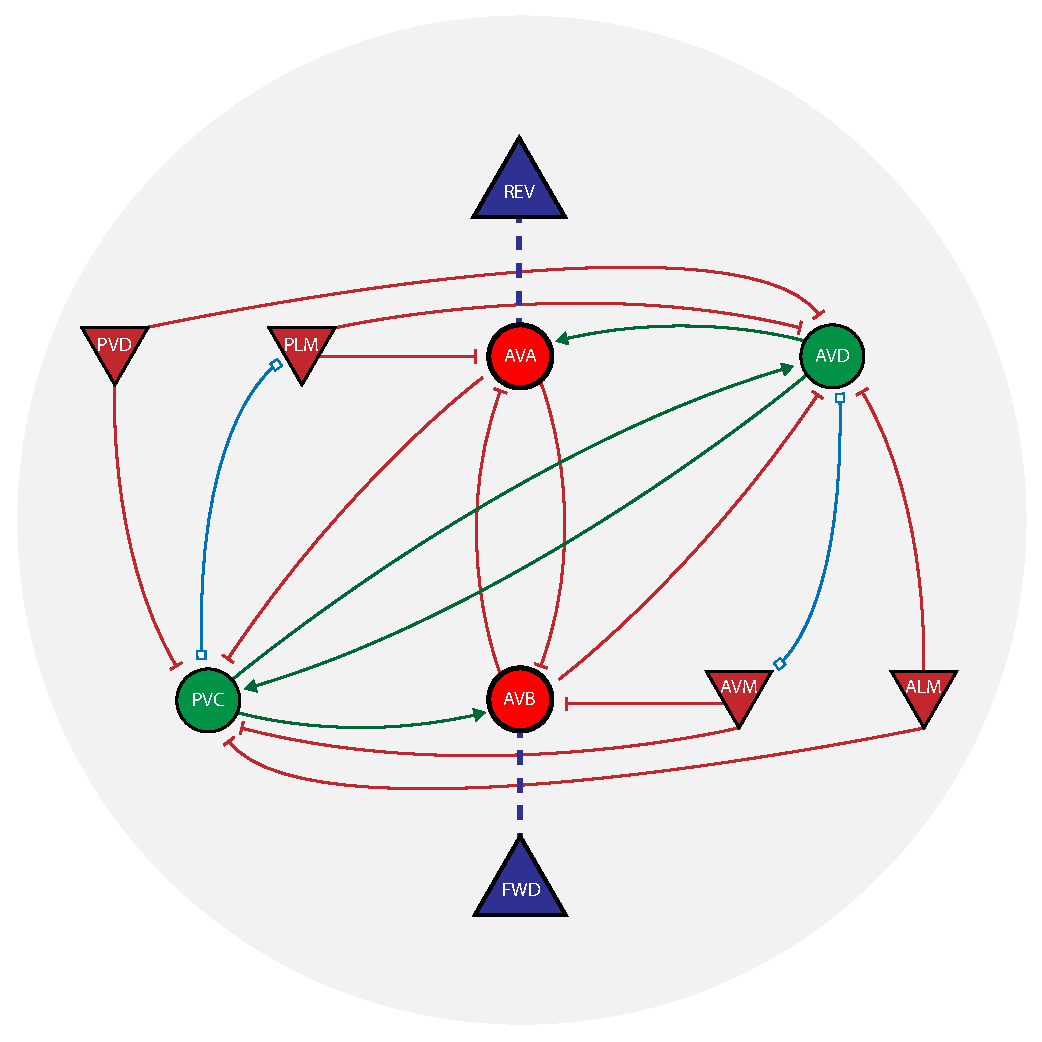
\includegraphics[width=4.5cm]{figures/folie_1/bnn.pdf}
		\btEmph{Biologische neuronale Netze}
	\end{column}
	\hspace{0.2cm}
	\begin{column}{0.3\textwidth}
		\centering
		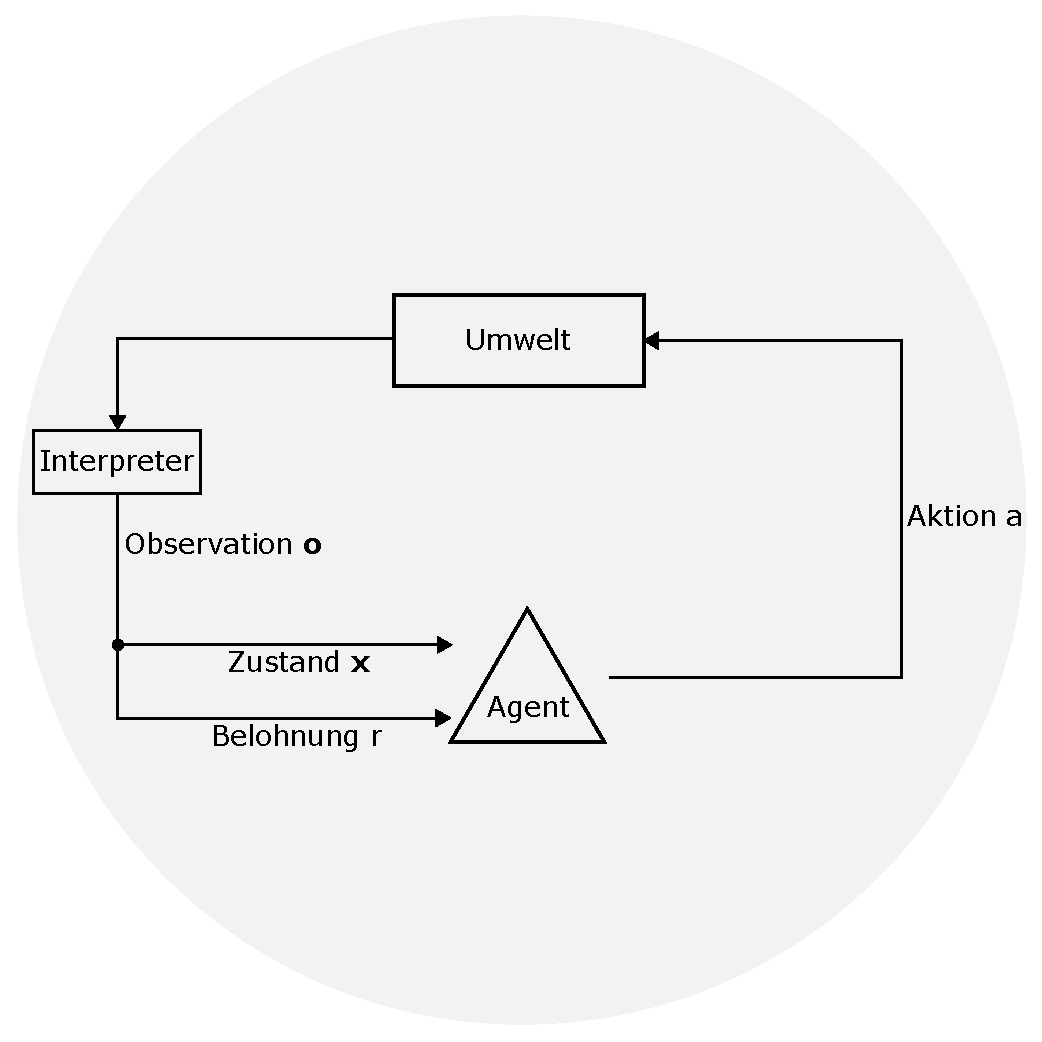
\includegraphics[width=4.5cm]{figures/folie_1/rl.pdf}
		\btEmph{Reinforcement Learning}
	\end{column}
	\hspace{0.2cm}
	\begin{column}{0.3\textwidth}
		\centering
		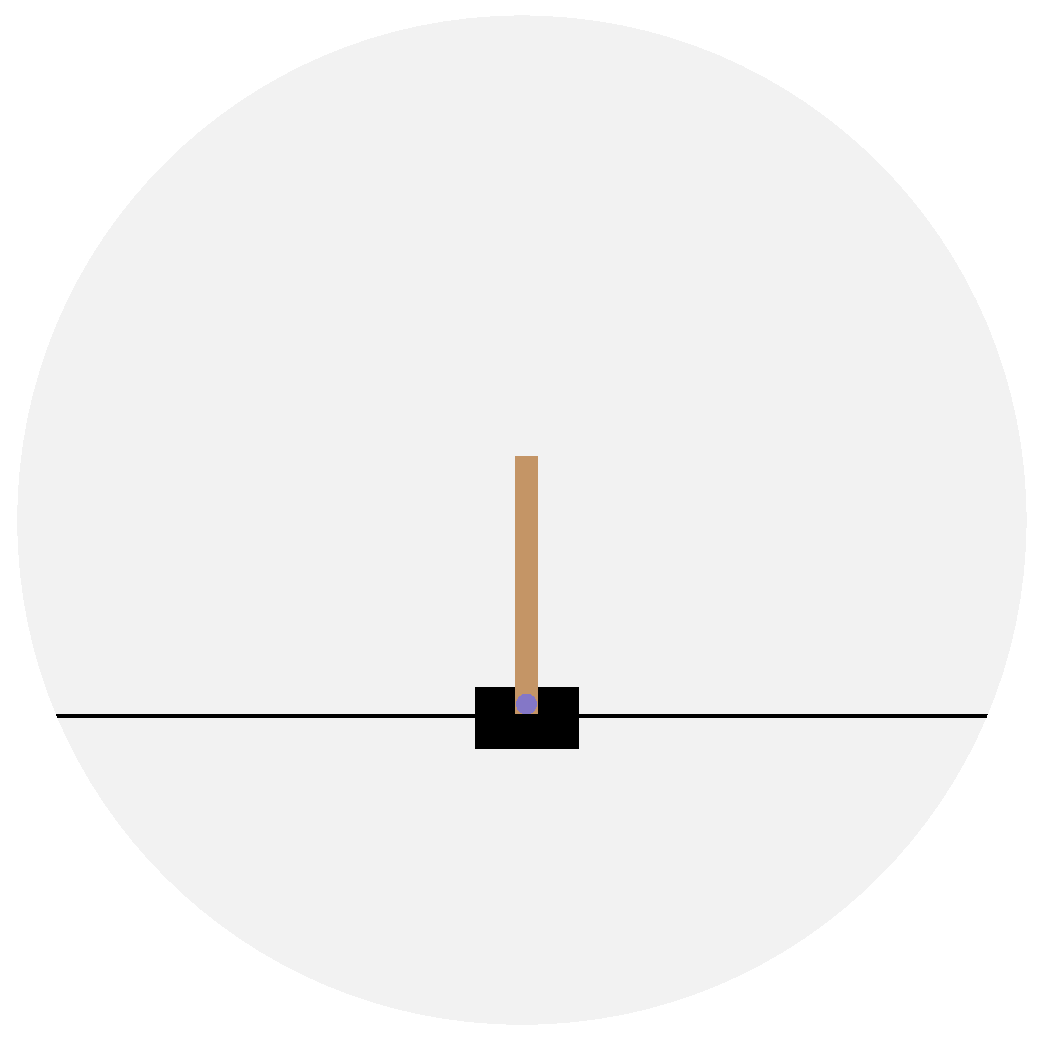
\includegraphics[width=4.5cm]{figures/folie_1/cartpole.pdf}
		\btEmph{Simulation: inverses Pendel}
	\end{column}
\end{columns}

\end{frame}

% =======================

\begin{frame}
	\frametitle{\Inhalt}
	\vspace{1cm}
	\begin{columns}[T,onlytextwidth]
		\begin{column}{0.45\textwidth}
			\centering
			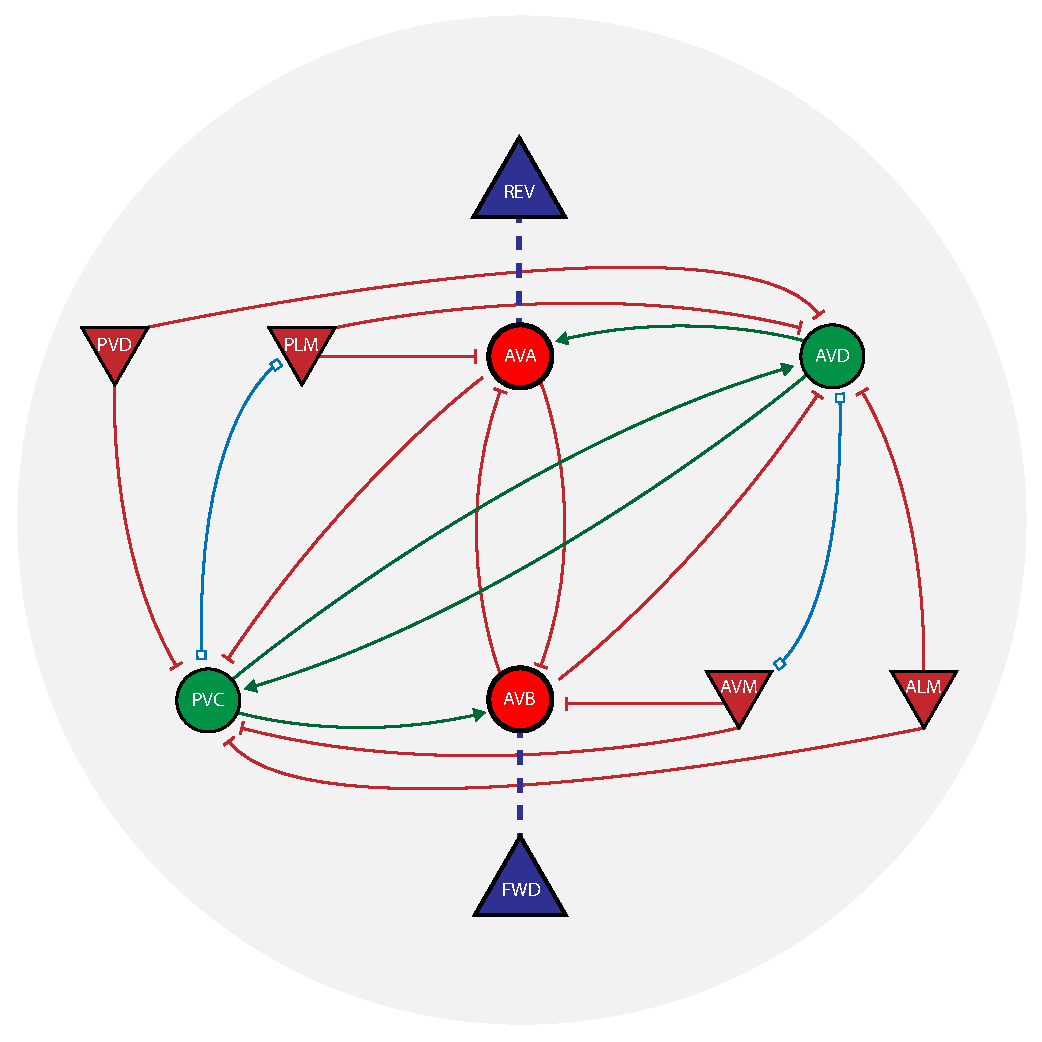
\includegraphics[width=4.5cm]{figures/folie_1/bnn.pdf}\\
			\btEmph{Biologische neuronale Netze}
		\end{column}
		\hspace{0.2cm}
		\begin{column}{0.45\textwidth}
			\vspace{0.8cm}
			\begin{itemize}
				\item[\IconArrow] Nervenzellen \& Synapsen\vspace{0.6cm}
				\item[\IconArrow] Biologisches neuronales Netzwerk\vspace{0.6cm}
				\item[\IconArrow] Simulation neuronaler Dynamik
			\end{itemize}
		\end{column}
	\end{columns}
\end{frame}

% =======================

\begin{frame}
	\frametitle{\ChapterBnn}
	\framesubtitle{Biologische Nervenzellen}
	\vspace{0.3cm}
	Neuronale Netze biologischer Lebensformen bestehen aus Nervenzellen und Synapsen bzw. Gap-Junctions.
	\vspace{0.2cm}
	\begin{itemize}
		\item Der \textbf{Dendrit} dient der Reizaufnahme von Signalen anderer Nervenzellen übertragen durch Synapsen und Gap-Junctions.
		\item Das \textbf{Soma} enthält den Zellkern und verarbeitet ankommende Informationen.
		\item Das \textbf{Axon} ist ein Nervenzellenfortsatz zur Weiterleitung der Signale von Soma an weitere Synapsen und Gap-Junctions.
	\end{itemize}
	\begin{figure}[H] %[!t] ...
		\centering
		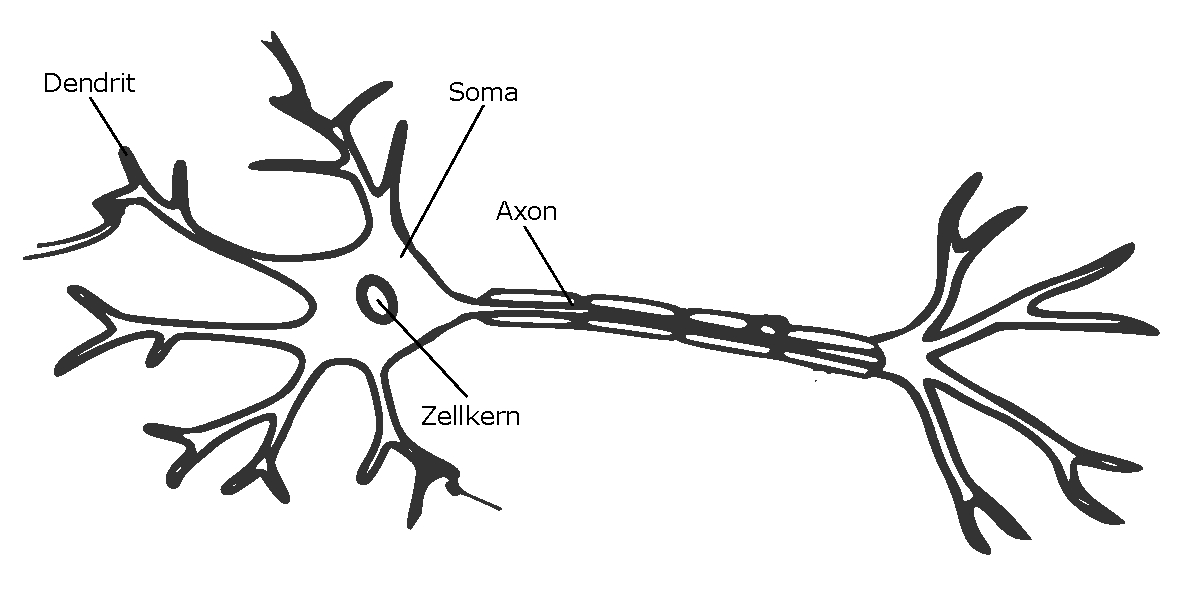
\includegraphics[width=7.2cm]{figures/folie_2/neuron_is.pdf}
		\label{fig:neuron}
	\end{figure}

\end{frame}

% =======================

\begin{frame}
	\frametitle{\ChapterBnn}
	\framesubtitle{Biologische Synapsen}
	\vspace{0.3cm}
	Eine Synapse dient der Informationsübertragung zwischen zwei Nervenzellen und wird in drei Kategorien unterteilt:
	\vspace{0.2cm}
	\begin{itemize}
		\item Exzitatorische Synapsen (chemisch) - wirken anregend auf die postsynaptische Nervenzelle und übertragen die Informationen.
		\item Inhibitorische Synapse (chemisch) - wirken  hemmend auf die postsynaptische Nervenzelle und übertragen die Informationen negativ.
		\item Gap-Junctions (elektrisch) - wirken bidirektional als synchronisierende Verbindung und gleichen Potentialunterschiede aus.
	\end{itemize}
	\begin{figure}[H] %[!t] ...
		\centering
		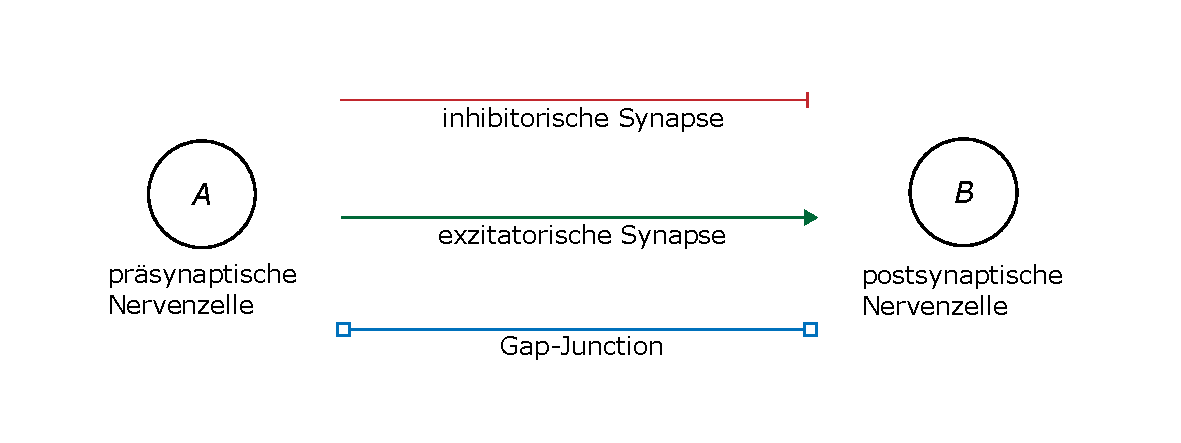
\includegraphics[width=8cm]{figures/folie_3/synapse_is.pdf}
		\label{fig:synapse}
	\end{figure}

\end{frame}

% =======================

\begin{frame}
	\frametitle{\ChapterBnn}
	\framesubtitle{Biologisches neuronales Netz des \textit{C. Elegans}}
	\vspace{0.3cm}
	Der \textit{Touch-Withdrawal Circuit} des \textit{C. Elegans} dient des reflexartigen Zurückschnellens bei äußeren Stimuli.
	\begin{columns}[T,onlytextwidth]
		\begin{column}{0.58\textwidth}
			\begin{itemize}
				\item[\SensorNeuron] \textbf{Sensor-Neuronen} nehmen Signale durch äußere Stimuli auf und übersetzen diese auf Aktions-\\potentiale innerhalb des neuronalen Netzes.\vspace{0.3cm}
				\item[\InterNeuron] \textbf{Inter-Neuronen} nehmen durch Synapsen und Gap-Junctions Akionspotentiale entgegen und summieren diese auf, bis ein Schwellwert erreicht wird und es feuert.\vspace{0.3cm}
				\item[\MotorNeuron] \textbf{Motor-Neuronen} sorgen bei entsprechenden Feuer-Events für die Anregung von Muskelgruppen, um bspw. eine Vorwärtsbewegung umzusetzen.
			\end{itemize}
		\end{column}
		\hspace{0.2cm}
		\begin{column}{0.43\textwidth}
			\vspace{-0.7cm}
			\begin{figure}[H] %[!t] ...
				\centering
				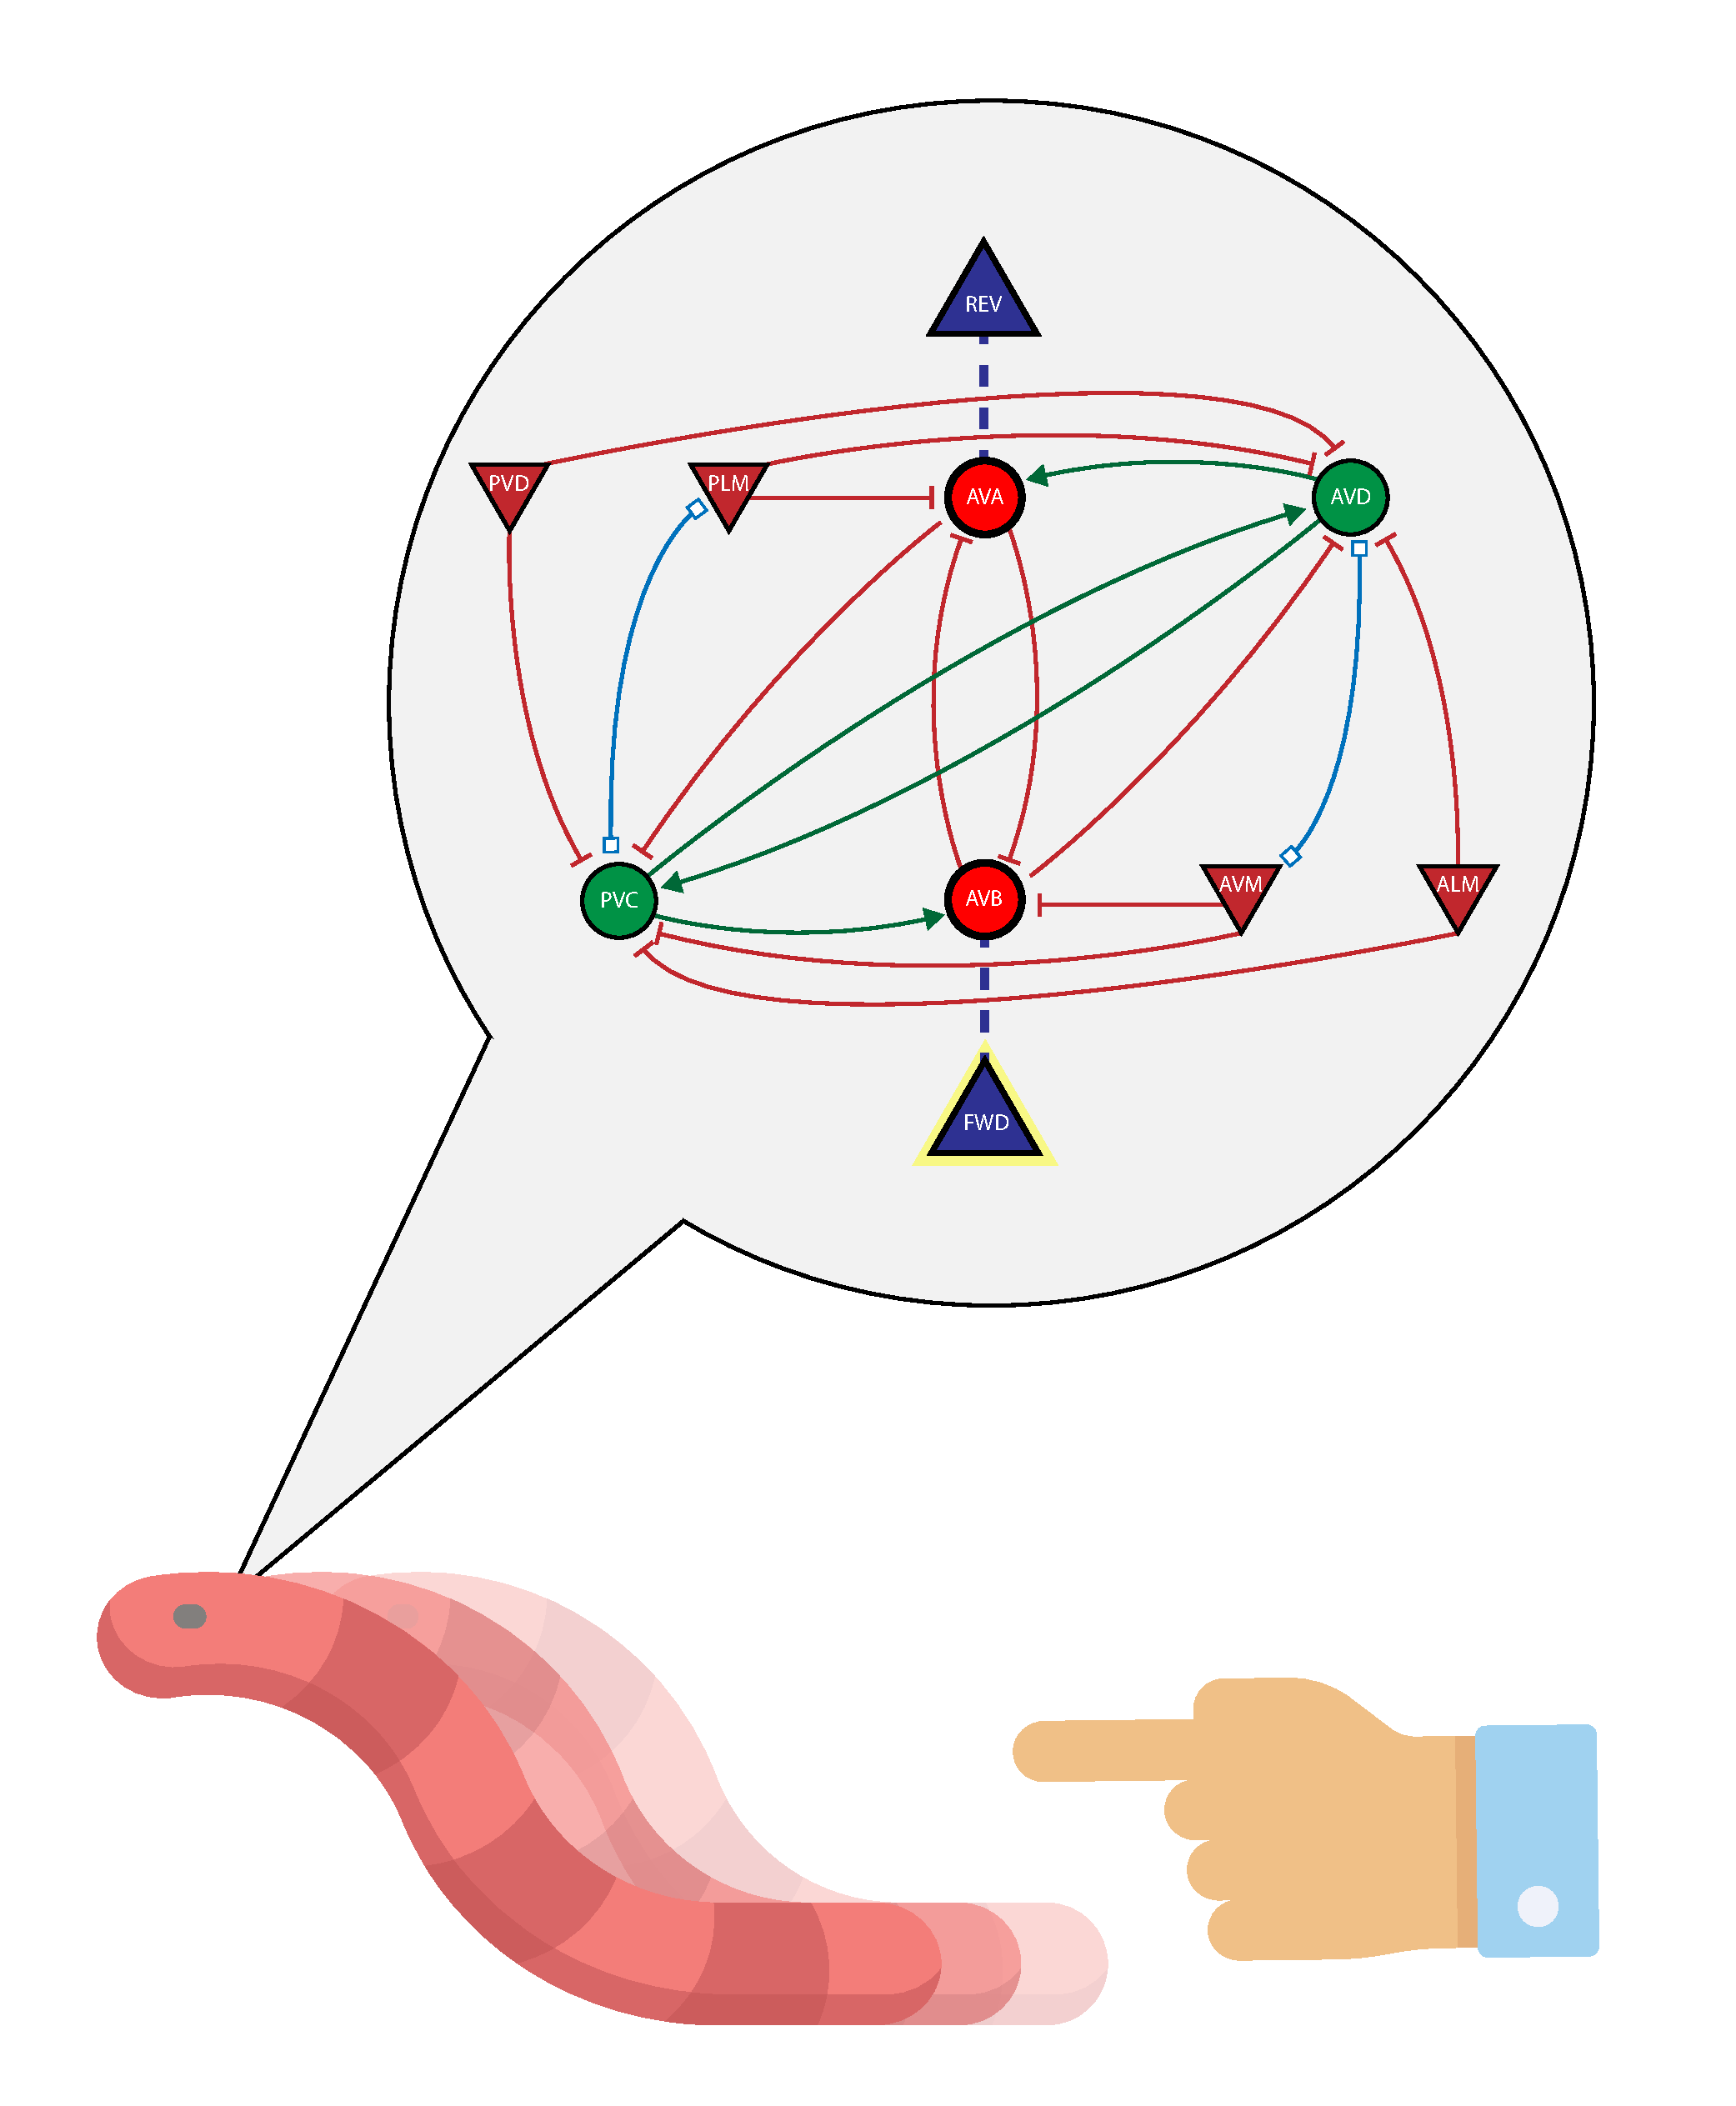
\includegraphics[width=5.5cm]{figures/nn_with_worm.pdf}
				\label{fig:symm_nn}
			\end{figure}
		\end{column}
	\end{columns}
\end{frame}

% =======================

\begin{frame}
	\frametitle{\ChapterBnn}
	\framesubtitle{Neuronale Dynamik durch das Leaky Integrate and Fire - Modell}
	\vspace{0.3cm}
	Die neuronale Dynamik und die damit verbundenen Vorgänge im neuronalen Netz werde durch das \textit{Leaky Integrate and Fire (LIF)} - Modell dargestellt.
	\begin{columns}[T,onlytextwidth]
		\begin{column}{0.55\textwidth}
			\vspace{0.1cm}
			\begin{alignbox}{0.9\textwidth}
				Berechnung des Membranpotentials bei anliegenden Synapsen- und Gap-Junction-Strömen:\\
				\begin{align}
					\label{eq:lif}
					\frac{dU}{dt} &= \frac{G_{Leak}(U_{Leak} - U) + I_{in}}{C_m}\text{ mit}\\
					\label{eq:lif_current_in}
					I_{in} &= \sum_{i = 1}^{n}{I_{Stimuli}} + \sum_{i = 1}^{n}{I_{Syn}} + \sum_{i = 1}^{n}{I_{Gap}}\text{.}
				\end{align}
			\end{alignbox}\\
			\vspace{0.3cm}
			\begin{alignbox}{0.9\textwidth}
				Berechnung der Synapsen- und Gap-Junction-Ströme:\\	
				\begin{align}
					\label{eq:chem_syn_current}
					I_{Syn} &= \frac{\omega}{1 + \exp^{\sigma(u_{pre} + \mu)}}(E - u_{post}),\\
					\label{eq:gap_syn_current}
					I_{Gap} &= \hat{\omega}(u_{post} - u_{pre})\text{.}
				\end{align}
			\end{alignbox}
		\end{column}
		\hspace{0.2cm}
		\begin{column}{0.45\textwidth}
			\vspace{0.5cm}
			\begin{figure}
				\centering
				\begin{circuitikz}
					\draw
					(0,4) to [short, o-*] (1,4)
					to [generic, l=$R$] (1,2)
					to [battery1, l=$U_{Leak}$] (1,0)
					to [short, -*] (1,0)
					to [short, -o] (0,0)
					
					(1,4) to [short, i_>=$I$] (3,4)
					to [short, -*] (3,4)
					to [C, l=$C_m$] (3,0)
					to [short, -*] (3,0)
					to [short, -*] (1,0)
					
					(3,4) to [short, -o] (4,4)
					(3,0) to [short, -o] (4,0)
					(4,0) to [open, v_<=$U$] (4,4);
				\end{circuitikz}
				\caption{Ersatzschaltbild der Zellmembran}
				\label{cic:lif}
			\end{figure}
		\end{column}
	\end{columns}
\end{frame}

% =======================

\begin{frame}
	\frametitle{\ChapterBnn}
	\framesubtitle{Motivation: Nutzung eines biologischen neuronalen Netzes}
	\vspace{0.5cm}
	Klassische Anwendungen des \textit{Deep Learning} durch neuronale Netze stützen sich auf künstlich erstellte Modelle. Die Nutzung bereits bestehender Netzwerke birgt einige Vorteile:
	\vspace{0.5cm}
	\begin{columns}[T,onlytextwidth]
		\begin{column}{0.45\textwidth}
			\begin{itemize}
				\item[\IconPro] Profitieren von natürlicher Evolution.\vspace{0.5cm}
				\item[\IconPro] Starke Anpassungsfähigkeit durch zwei Eingängen und einem Ausgang.\vspace{0.5cm}
				\item[\IconPro] Einfache Erweiterbarkeit und Ausbau des Netzwerks durch Lernalgorithmen.\vspace{0.5cm}
				\item[\IconPro] Kurze Trainingsphasen.\vspace{0.5cm}
			\end{itemize}
		\end{column}
		\hspace{0.2cm}
		\begin{column}{0.45\textwidth}
			\begin{itemize}
				\item[\IconCon] Implementationsaufwand für die Simulation durch \textit{LIF}-Modell hoch.\vspace{0.5cm}
				\item[\IconCon] Wenig Fachliteratur über die Verbindung von biologischen neuronalen Netzen mit Methoden des Reinforcement Learning.\vspace{0.5cm}
				\item[\IconCon] Hohe Anzahl an zu simulierenden Parametern und ressourcenintensive Simulationen durch numerische Lösungsverfahren.\vspace{0.5cm}
			\end{itemize}
		\end{column}
	\end{columns}

\end{frame}

% =======================

\begin{frame}
\frametitle{\Inhalt}
\vspace{1cm}
\begin{columns}[T,onlytextwidth]
	\begin{column}{0.45\textwidth}
		\centering
		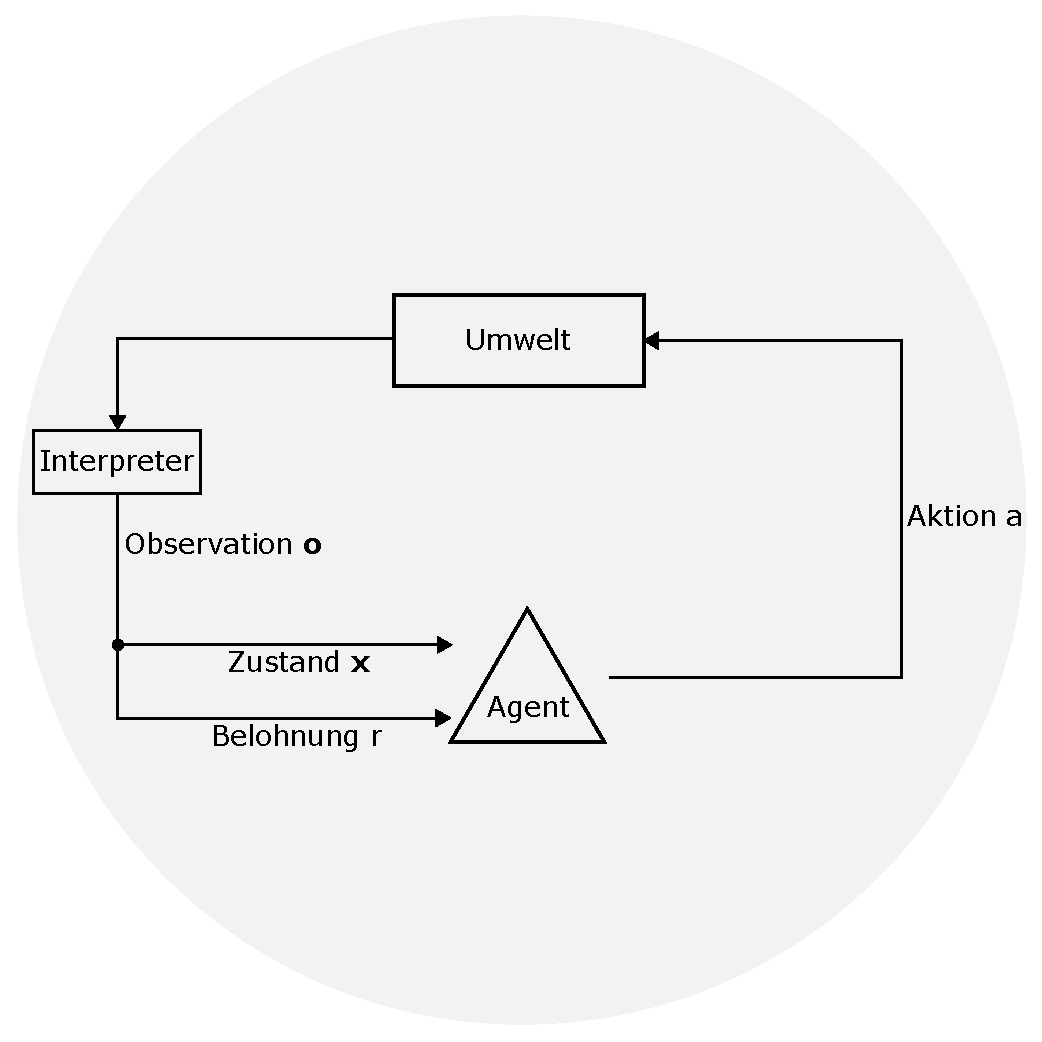
\includegraphics[width=4.5cm]{figures/folie_1/rl.pdf}\\
		\btEmph{Reinforcement Learning}
	\end{column}
	\hspace{0.2cm}
	\begin{column}{0.45\textwidth}
		\vspace{0.4cm}
		\begin{itemize}
			\item[\IconArrow] Deep Learning und Grundlagen von Lernalgorithmen\vspace{0.6cm}
			\item[\IconArrow] Vorteile des Belohnungssystems\vspace{0.6cm}
			\item[\IconArrow] Reinforcement Learning durch Random-Search und genetischen Algorithmen
		\end{itemize}
	\end{column}
\end{columns}
\end{frame}

% =======================

\begin{frame}
	\frametitle{\ChapterRl}
	\framesubtitle{Reinforcement Learning und das Belohnungssystem}
	\vspace{0.3cm}
	\textit{Reinforcement Learning} aus dem Bereich des \textit{Deep Learning} ist eine Abwandlung des überwachten Lernens mit der Erweiterung eines Belohnungssystems.
	\begin{columns}[T,onlytextwidth]
		\begin{column}{0.5\textwidth}
			\vspace{0.2cm}
			\begin{itemize}
			  \item Der Agent ist in der Lage, eine Aktion im gegebenen Aktionsraum zu tätigen.
			  \item Die Aktion hat Auswirkungen auf die Umwelt bzw. Simulation, der neue Zustand der Simulation wird interpretiert und als Observationsvektor $\boldsymbol{o}$ ausgegeben.
			  \item Aus der Observation $\boldsymbol{o}$ gehen zum einen der Zustandsvektor $\boldsymbol{x}$ zum anderen die Belohnung $r$ hervor.
			  \item Diese Größen werden von dem Agenten interpretiert und dienen als neue Entscheidungsgrundlage der nächsten Aktion.
			\end{itemize}
		\end{column}
		\hspace{-0.5cm}
		\begin{column}{0.45\textwidth}
			\vspace{1cm}
			\begin{figure}[H] %[!t] ...
				\centering
				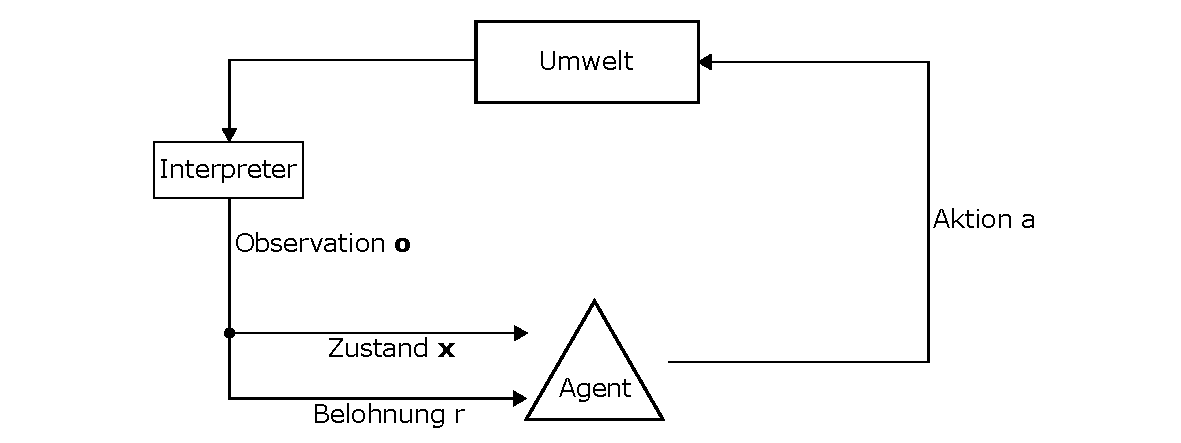
\includegraphics[width=8cm]{figures/RL_Chart_pres.pdf}
				\caption{Funktionweise des \textit{Reinforcement Learning}}
				\label{fig:rl}
			\end{figure}
		\end{column}
	\end{columns}
\end{frame}

% =======================

\begin{frame}
	\frametitle{\ChapterRl}
	\framesubtitle{Anwendung auf das biologische Netzwerk}
	\vspace{0.3cm}
	Durch \textit{Reinforcement Learning} können Parameter im biologischen neuronalen Netz optimiert werden, sodass es zu Feuer-Events kommt und ein gegebenes System stabilisiert werden kann.
	\vspace{0.2cm}
	\begin{columns}[T,onlytextwidth]
		\begin{column}{0.5\textwidth}
			\begin{itemize}
				\item Es werden insgesamt 46 Parameter generiert und optimiert, um die neuronale Dynamik richtig abzubilden.
				\item Die Belohnung nach jeder Episode (Simulationslauf eines bestimmten Parametersatzes) gibt Aufschluss über die Güte der generierten Parameter.
				\item Es erfolgt eine nachgelagerte Optimierung durch weitere Gewichtung der Synapsen und Gap-Junctions.
			\end{itemize}
		\end{column}
		\hspace{1cm}
		\begin{column}{0.45\textwidth}
			\vspace{-0.5cm}
			\begin{figure}[H] %[!t] ...
				\centering
				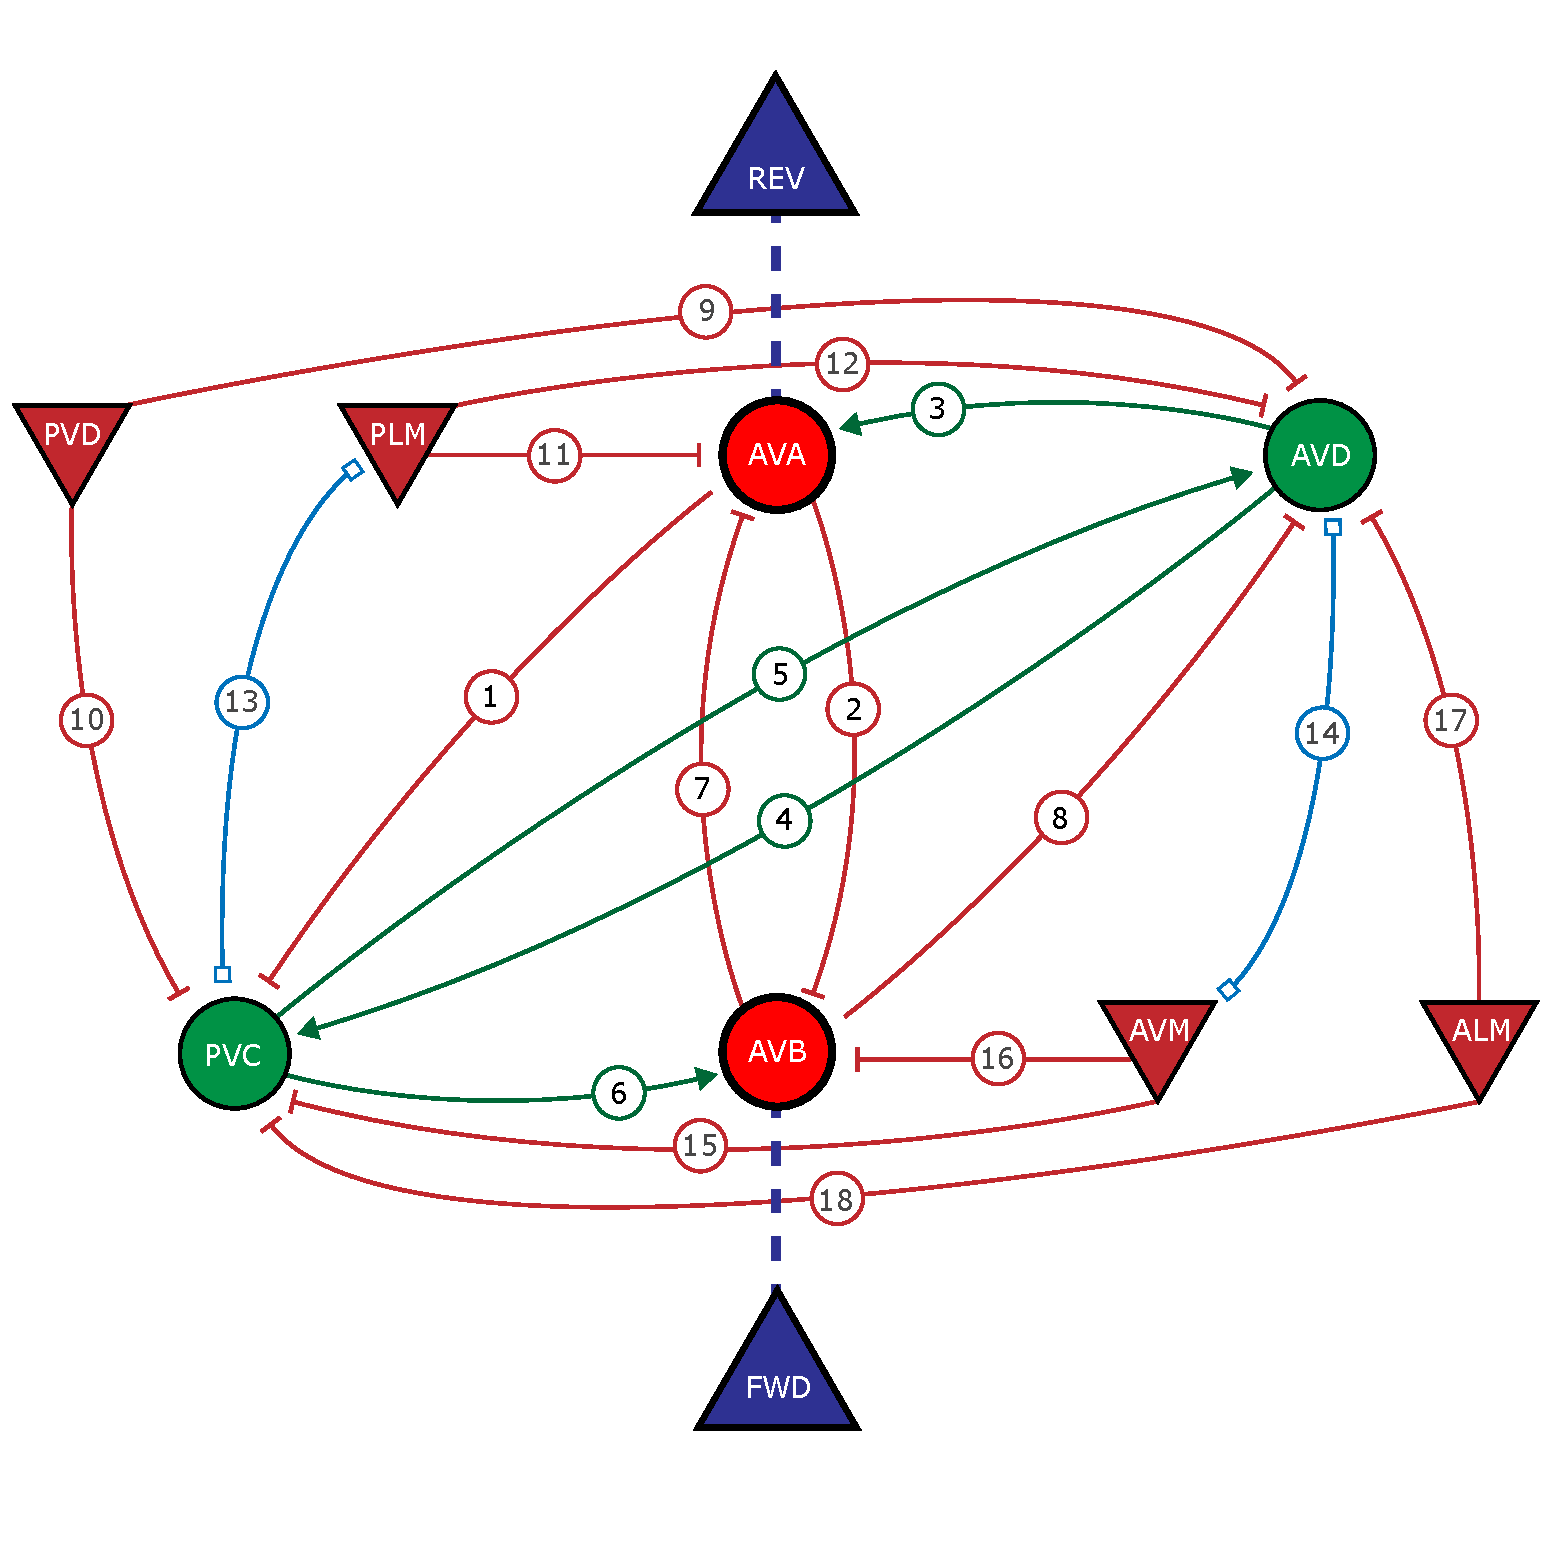
\includegraphics[width=5cm]{figures/Neural_Net_v3_num_syn.pdf}
				\caption{Biologisches neuronales Netzwerk mit Synapsengewichtung.}
				\label{fig:bnn_num}
			\end{figure}
		\end{column}
	\end{columns}
\end{frame}

% =======================

\begin{frame}
	\frametitle{\ChapterRl}
	\framesubtitle{Suchalgorithmen}
	\vspace{0.3cm}
	\begin{columns}[T,onlytextwidth]
		\begin{column}{0.5\textwidth}
			\btEmph{\texttt{Random-Search}}
			\vspace{0.1cm}
			\begin{itemize}
				\item Parameter werden in einer gegebenen Gleichverteilung mit festen Grenzen pro Episode zufällig generiert.
				\item Die Güte jedes Parametersatzes wird anhand der erhaltenen Belohnung gemessen.
				\item Nach Ablauf der Simulationszeit werden die Parameter gespeichert, welche die höchste Belohnung erhalten haben.
				\item[\IconArrow] Erfolgswahrscheinlichkeit hoch
				\item[\IconArrow] Ressourcenaufwand hoch
			\end{itemize}
		\end{column}
		\begin{column}{0.5\textwidth}
			\btEmph{\texttt{Weights}}
			\vspace{0.1cm}
			\begin{itemize}
				\item Der Algorithmus Weights wird zur Optimierung des neuronalen Netzes mit bereits bestehenden Parametern verwendet.
				\item Es werden bestehende Synapsen mit einem pro Episode zufällig gewählten Gewicht versehen.
				\item Die Güte der Gewichte wird ebenfalls anhand der erhaltenen Belohnung gemessen.
				\item Nach Ablauf der Simulationszeit werden die Gewichte gespeichert, welche die höchste Belohnung erhalten haben.
				\item[\IconArrow] Erfolgswahrscheinlichkeit hoch
				\item[\IconArrow] Ressourcenaufwand hoch
			\end{itemize}
		\end{column}
	\end{columns}
\end{frame}

% =======================

\begin{frame}
\frametitle{\ChapterRl}
\framesubtitle{Suchalgorithmen}
\vspace{0.3cm}
\begin{columns}[T,onlytextwidth]
	\begin{column}{0.5\textwidth}
		\btEmph{\texttt{Genetische Algorithmen}}
		\vspace{0.1cm}
		\begin{itemize}
			\item Die erste Generation an Parametern wird in einer gegebenen Gleichverteilung mit festen Grenzen pro Episode zufällig generiert.
			\item Nach Durchlauf der ersten Generation werden wenige Episoden mit guter Belohnung in eine Selektion aufgenommen.
			\item Die Grenzen der Gleichverteilung werden entsprechend der Maxima/Minima der Selektion angepasst.
			\item Die Simulation konvergiert auf ein lokales Belohnungs-Maximum für jeden Parameter.
		\end{itemize}
	\end{column}
	\begin{column}{0.45\textwidth}
		\begin{figure}[H] %[!t] ...
			\centering
			\scriptsize
			\def\svgwidth{6.3cm}
			\input{figures/gen_alg.pdf_tex}
			\caption{Grafische Darstellung des genetischen Algorithmus.}
			\label{fig:gen_alg}
		\end{figure}
	\end{column}
\end{columns}
\end{frame}

% =======================


\begin{frame}
\frametitle{\Inhalt}
\vspace{1cm}
\begin{columns}[T,onlytextwidth]
	\begin{column}{0.45\textwidth}
		\centering
		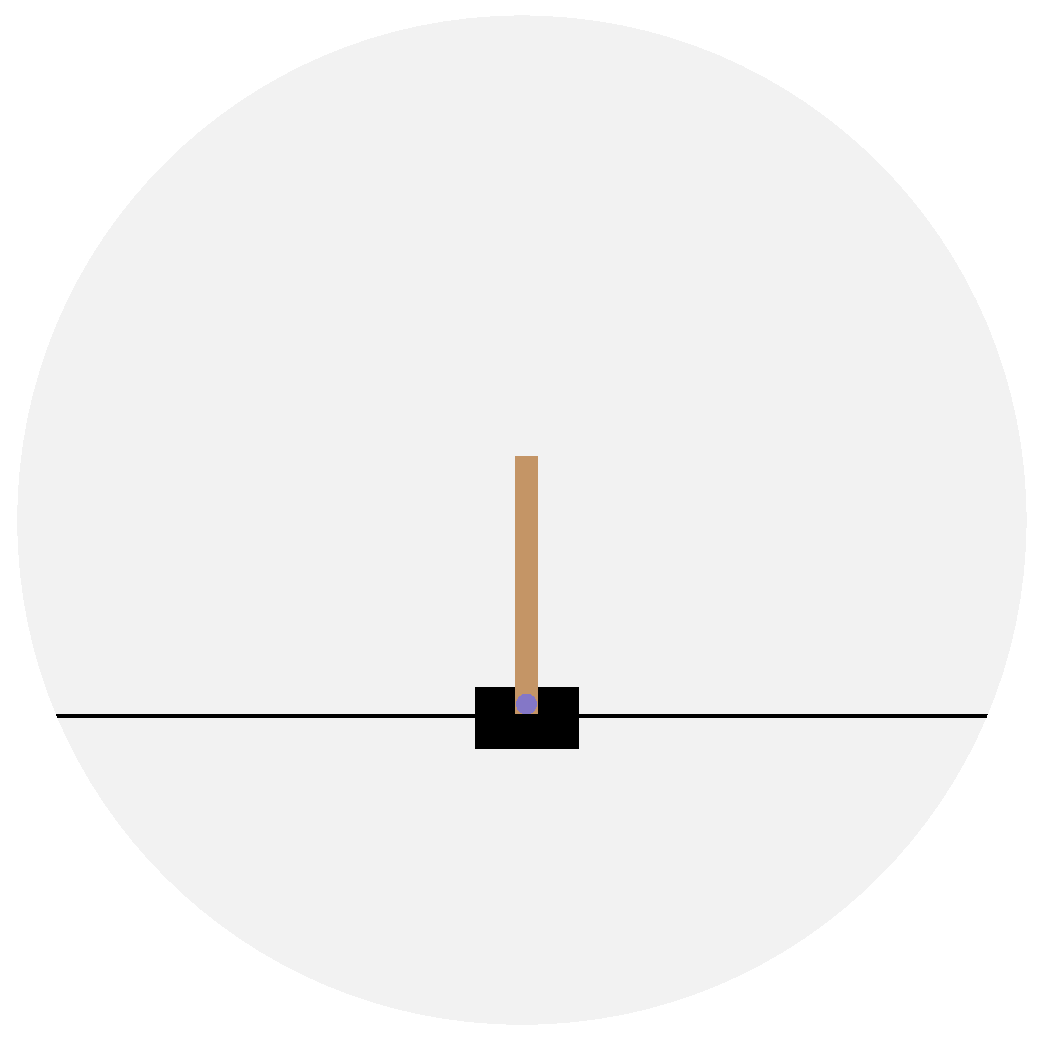
\includegraphics[width=4.5cm]{figures/folie_1/cartpole.pdf}\\
		\btEmph{Simulation: inverses Pendel}
	\end{column}
	\hspace{0.2cm}
	\begin{column}{0.45\textwidth}
		\vspace{0.8cm}
		\begin{itemize}
			\item[\IconArrow] Implementiertung des Simulators\vspace{0.6cm}
			\item[\IconArrow] Simulationsumgebung: OpenAI Gym\vspace{0.6cm}
			\item[\IconArrow] Grafische Darstellung und Auswertung der Simulation
		\end{itemize}
	\end{column}
\end{columns}
\end{frame}

% =======================



\begin{frame}
\frametitle{\ChapterCartpole}
\framesubtitle{Aufbau des Simulators}
\vspace{0.3cm}
\begin{columns}[T,onlytextwidth]
	\begin{column}{0.7\textwidth}
		Um die neuronale Dynamik des biologischen neuronalen Netzes zu simulieren und die Aktionen auf die Umwelt zu übertragen, wurde ein Simulator in der Programmiersprache \texttt{Python} geschrieben.
		\vspace{0.1cm}
		\begin{itemize}
			\item Wichtige Programmfunktonen werden in Modulen zusammengefasst und sind uneingeschränkt aufrufbar.
			\item Es existiert ein zentraler Punkt zum Ändern von Parametern des neuronalen Netzes sowie anderer Simulationsvariablen.
			\item Parameter und Gewichte werden nach Simulationen mit entsprechenden Informationen gespeichert und sind plattformunabhängig aufrufbar.
			\item Der Programmcode ist ausführlich kommentiert und es wurde eine entsprechende Dokumentation verfasst, um den Simulator nach eigenen Anforderungen zu erweitern.
		\end{itemize}
	\end{column}
	\hspace{-0.8cm}
	\begin{column}{0.28\textwidth}
		\vspace{-0.7cm}
		\resizebox{4cm}{!} {
		\begin{forest}
			pic dir tree,
			where level=0{}{% folder icons by default; override using file for file icons
				directory,
			},
			[TW Circuit
			[docs]
			[information]
			[modules
			[genetic\_algorithm.py, file]
			[inspect.py, file]
			[lif.py, file]
			[parameters.py, file]
			[random\_search\_v2.py, file]
			[visiualize.py, file]
			[weights.py, file]]
			[parameter\_dumps]
			[weight\_dumps]
			[main.py, file]]
		\end{forest}
		}
	\end{column}
\end{columns}
\end{frame}

% =======================

\begin{frame}
	\frametitle{\ChapterCartpole}
	\framesubtitle{Simulationsumgebung \texttt{CartPole\_v0}}
	\vspace{0.3cm}
	Um die Methode des \textit{Reinforcement Learning} auf biologische neuronale Netze anzuwenden, wird die Simulationsumgebung \texttt{CartPole\_v0} von OpenAI Gym gewählt.
	\vspace{0.1cm}
	\begin{columns}[T,onlytextwidth]
		\begin{column}{0.53\textwidth}
			\begin{itemize}
				\item Das inverse Pendel auf dem Wagen kann sich in Vorwärts- und Rückwärtsrichtung bewegen.
				\item Pro Zeitschritt kann ein Schritt in die jeweilige Richtung erfolgen (Aktion: 0 oder 1).
				\item Der Observationsvektor $\boldsymbol{o}$ gibt die Zustandsgrößen $\varphi$, $\dot{\varphi}$, $x$ und $\dot{x}$ wieder.
				\item Es wird ebenfalls eine Belohnung $r$ zurückgegeben.
				\item Die Ein- bzw. Ausgangsgrößen werden mit den eingangs erwähnten Sensor- und Motor-Neuronen verbunden.
			\end{itemize}
		\end{column}
		\hspace{-0.5cm}
		\begin{column}{0.45\textwidth}
			\vspace{-0.6cm}
			\begin{figure}[H] %[!t] ...
				\centering
				\scriptsize
				\def\svgwidth{6.5cm}
				\input{figures/cartpole_with_ann.pdf_tex}
				\caption{Simulationsumgebung \texttt{CartPole\_v0}}
				\label{fig:cartpole}
			\end{figure}
		\end{column}
	\end{columns}
\end{frame}

% =======================

\begin{frame}
	\frametitle{\ChapterCartpole}
	\framesubtitle{Simulationsläufe: Auslagerung auf Cloud Server}
	\vspace{0.3cm}
	Durch rechenintensive Simulationen mit den Algorithmen \texttt{Random-Search} und \texttt{Weights} wird ein externer Server mit größeren Ressourcen benötigt.
	\vspace{0.1cm}
	\begin{columns}[T,onlytextwidth]
		\begin{column}{0.6\textwidth}
			\begin{itemize}
				\item Eine virtuelle Instanz in der Google Cloud Platform wurde angemietet, um Simulationszeiten über 12 Stunden zu ermöglichen.
				\item Es wurden Simulationen mit über 10 Mio. Episoden gefahren und analysiert.
				\item Die Ergebnisse dieser Simulationen werden in Form von Parameter- und Weight-\glqq Dumps\grqq{} bereitgestellt und können auf Heimrechnern visualisiert werden.
			\end{itemize}
			\begin{figure}[H] %[!t] ...
				\centering
				
\includegraphics[width=6cm]{figures/gcp.png}
				\label{fig:gcp}
			\end{figure}
		\end{column}
		\hspace{-0.5cm}
		\begin{column}{0.4\textwidth}
			\vspace{-0.6cm}
			\begin{figure}[H] %[!t] ...
				\centering
				\scriptsize
				\def\svgwidth{4cm}
				\input{figures/gcp/gcp.pdf_tex}
			\end{figure}
		\end{column}
	\end{columns}
\end{frame}

% =======================

\begin{frame}
	\frametitle{\ChapterCartpole}
	\framesubtitle{Visualisierung der Simulationsergebnisse}
	\vspace{0.3cm}
	Darstellung der Membranpotentiale über eine Simulationsdauer von 5 Sekunden:
	\vspace{-0.2cm}
	\begin{figure}[H] %[!t] ...
		\centering
		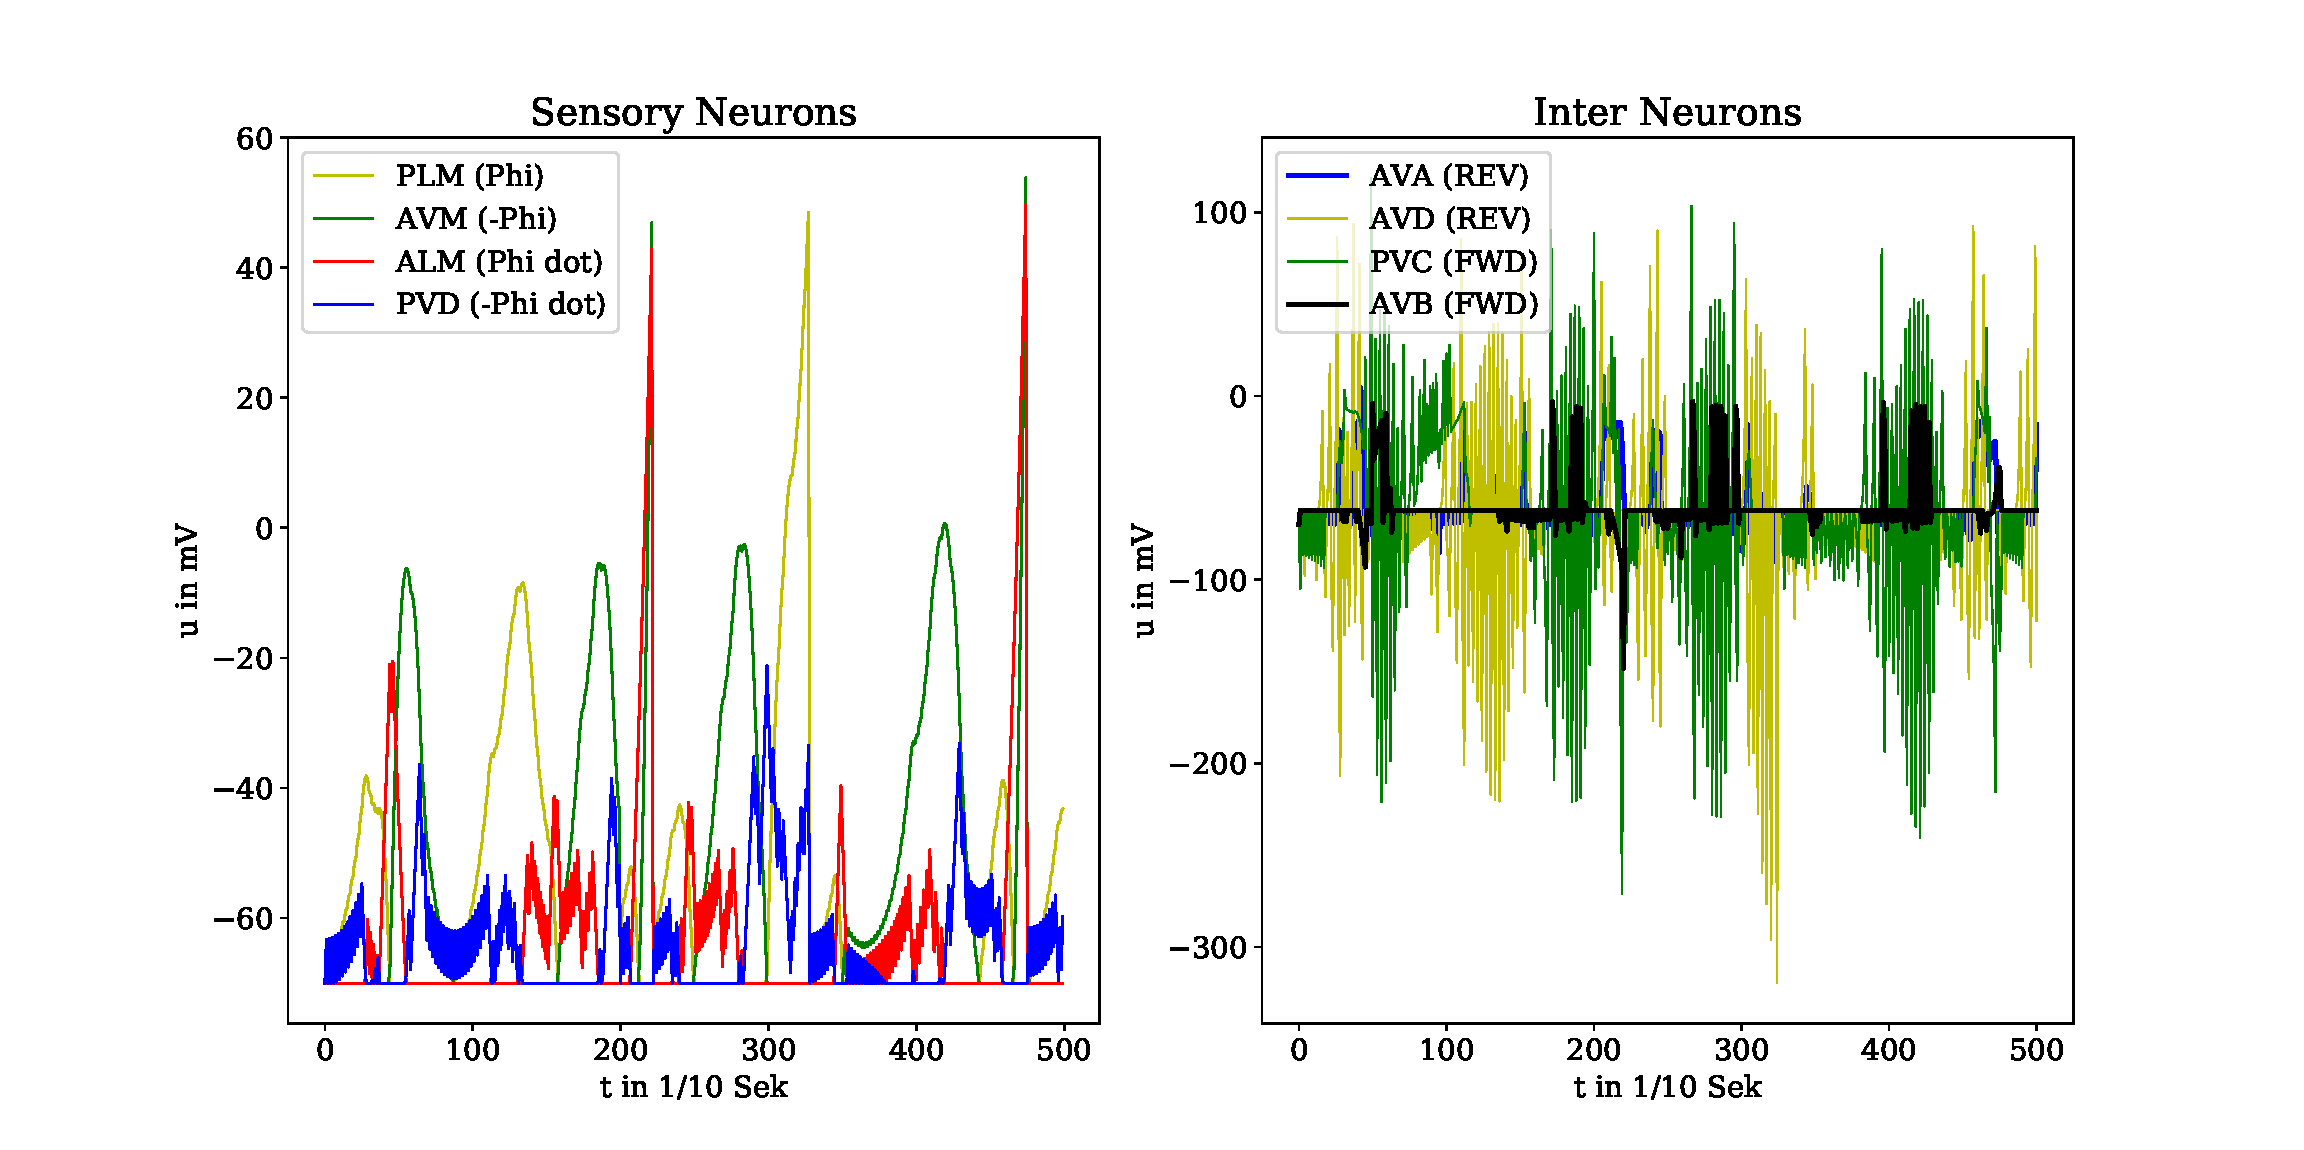
\includegraphics[width=14cm]{figures/plot_membranpot_2.pdf}
		\label{fig:memb_pot}
	\end{figure}
\end{frame}

% =======================

\begin{frame}
	\frametitle{\ChapterCartpole}
	\framesubtitle{Visualisierung der Simulationsergebnisse}
	\vspace{0.3cm}
	Darstellung der Aktion des neuronalen Netzes mit Winkel $\varphi$ des Pendels über eine Simulationsdauer von 5 Sekunden:
	\vspace{-0.2cm}
	\begin{figure}[H] %[!t] ...
		\centering
		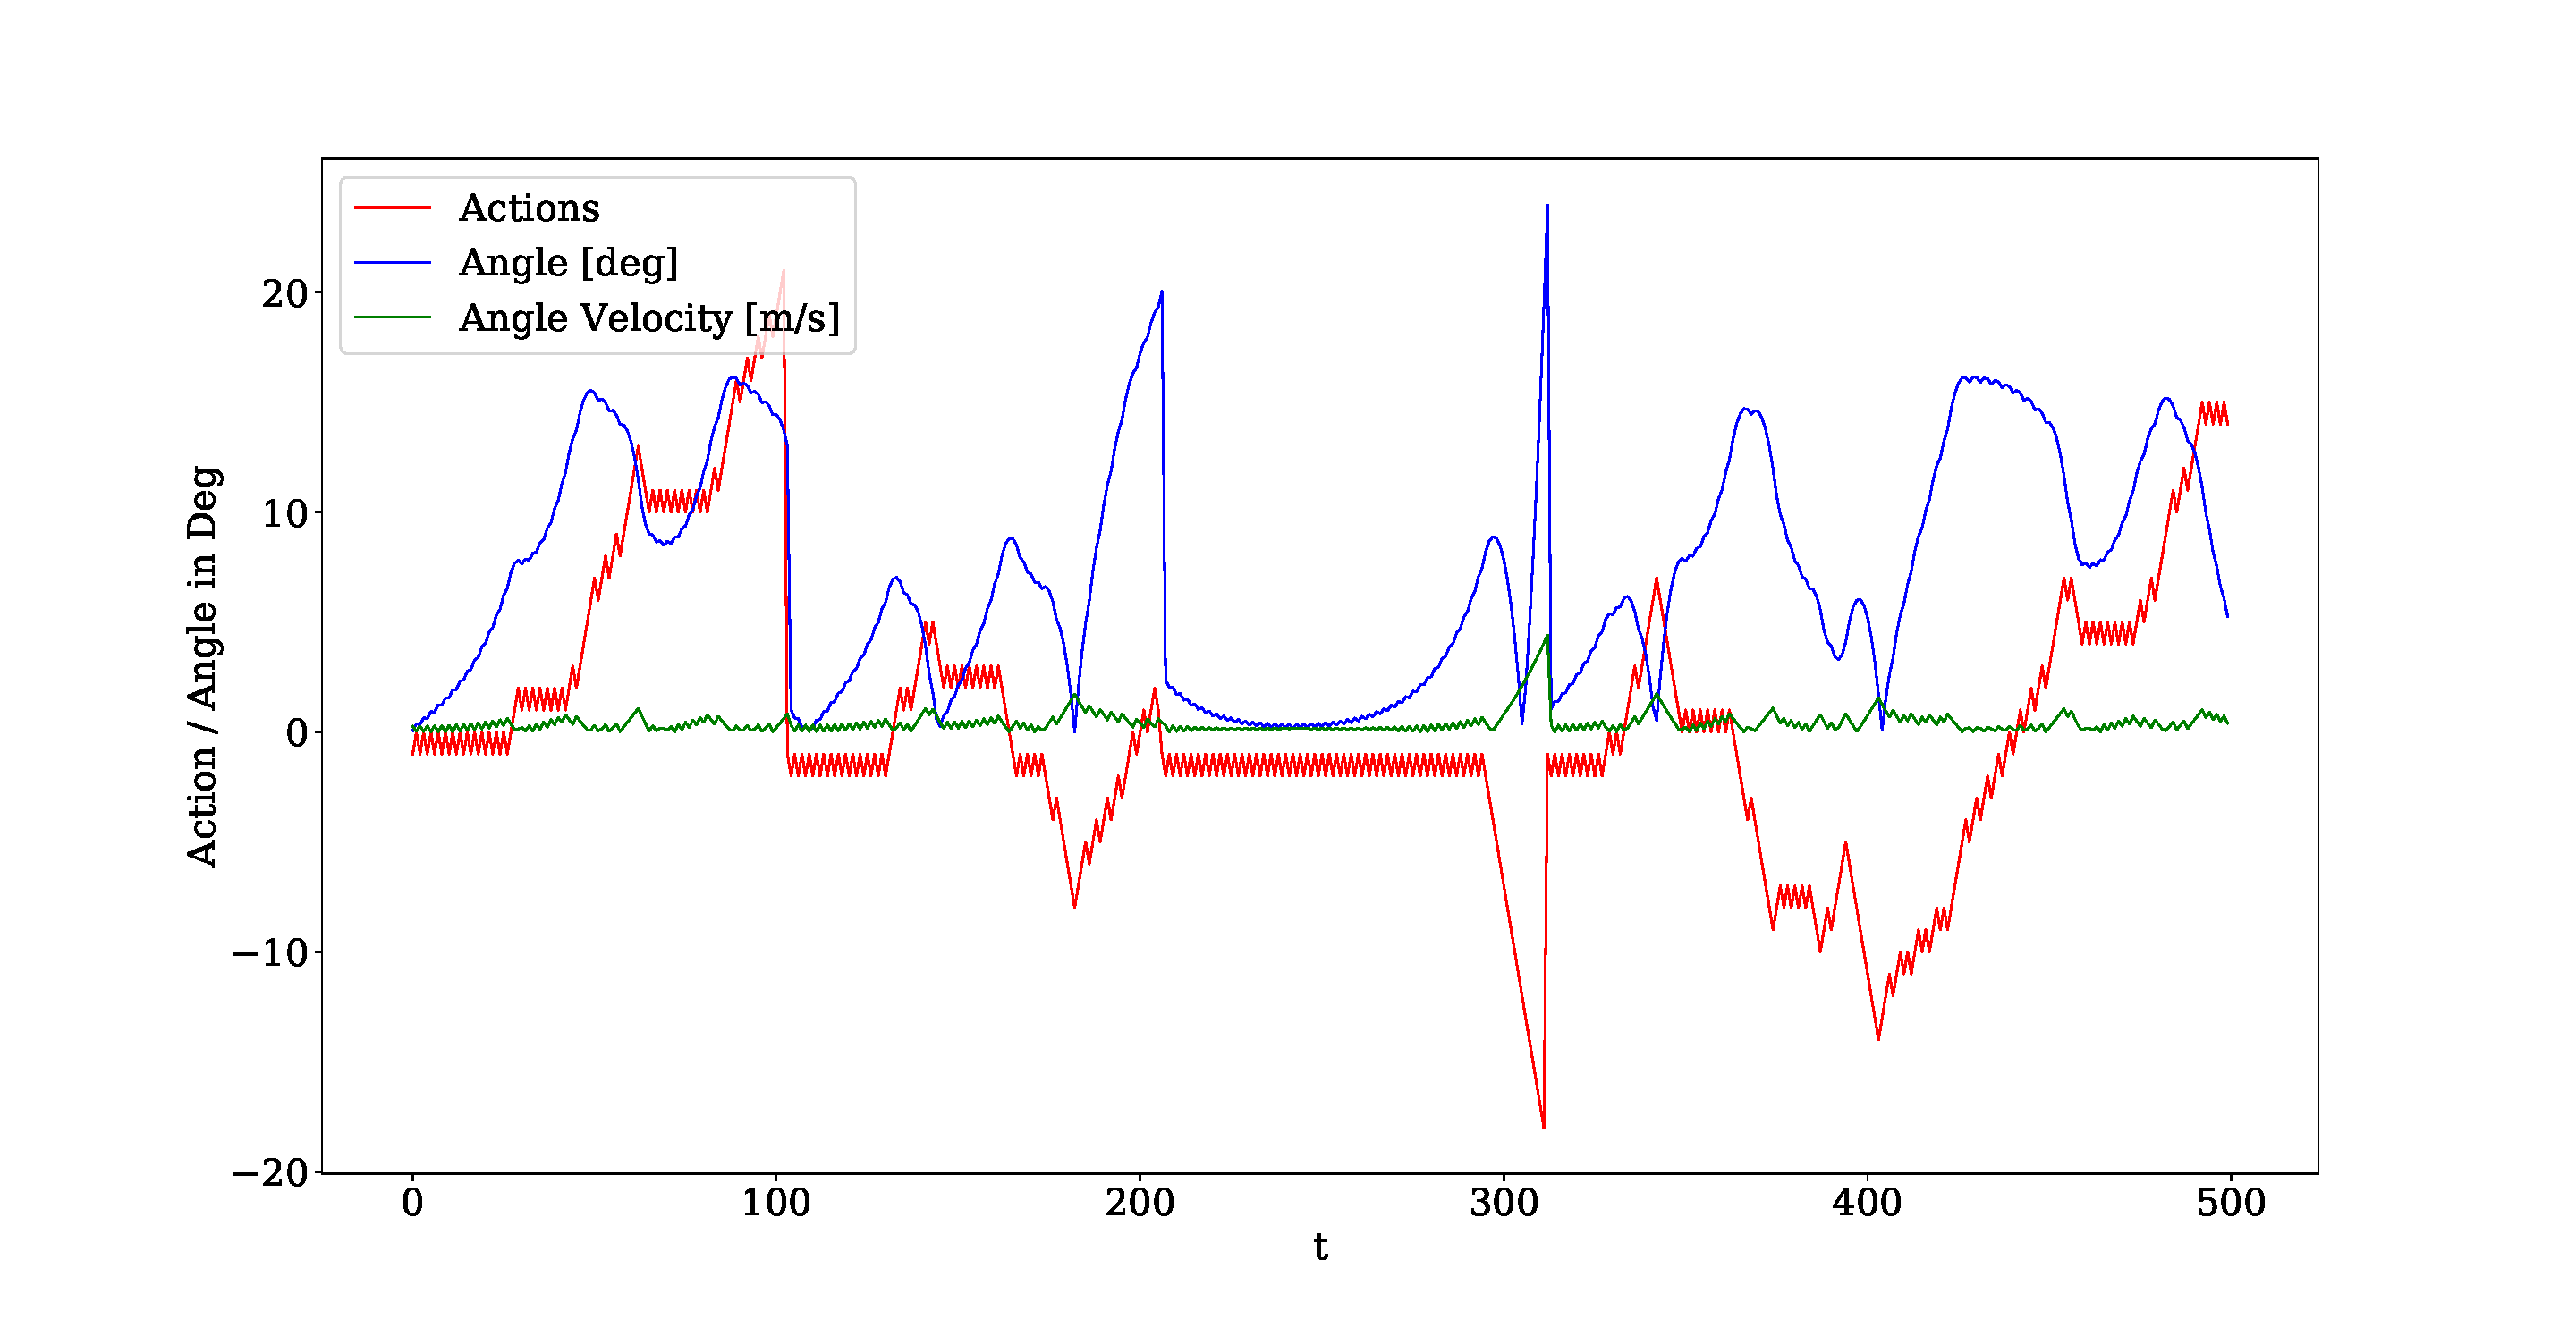
\includegraphics[width=13cm]{figures/plot_action.pdf}
		\label{fig:action}
	\end{figure}
\end{frame}

% =======================

\begin{frame}
	\frametitle{\ChapterCartpole}
	\framesubtitle{Simulation des inversen Pendels (Video)}
	\vspace{0.3cm}
	Das Video zeigt das inverse Pendel, welches durch das biologische neuronale Netz und bereits trainierten Parametern stabilisiert wird.\\
	\vspace{0.3cm}
		\centering
		\includemedia[
		width=14cm,height=6cm,
		activate=pageopen,
		addresource=video/20180910_Render_MP4.mp4,
		flashvars={
			source=video/20180910_Render_MP4.mp4
			&autoPlay=true
		}
		]{}{VPlayer.swf}

\end{frame}

% =======================

\begin{frame}
	\frametitle{\ChapterEnd}
	\framesubtitle{Zusammenfassung}
	\vspace{0.3cm}
	\begin{itemize}
		\item Ein Simulator für neuronale Dynamik wurde zur Simulation genereller Abläufe innerhalb eines biologischen neuronalen Netzes entwickelt. 
		\item Such- und Optimierungsalgorithmen im Bereich des \textit{Reinforcement Learning} sind implementiert worden, um die Parametersuche zu realisieren.
		\item Die Stabilisierung des inversen Pendels kann durch richtig gefundene Parameter bzw. Gewichte gewährleistet werden.
		\item Probleme treten in der Optimierung der Parameter sowie in der internen Verschaltung des gegebene neuronalen Netzes auf.
	\end{itemize}

\end{frame}

% =======================

\begin{frame}
\frametitle{\ChapterEnd}
\framesubtitle{Ausblick}
	\vspace{0.3cm}
	\begin{itemize}
		\item Durch den modularen Aufbau des Simulators kann dieser erweitert und verbessert werden.
		\item Die neuronale Dynamik kann durch erweiterte Modelle präziser dargestellt werden.
		\item Das gegebene neuronale Netz des \textit{C. Elegans} könnte durch erweiterte Literaturrecherche realitätsgetreuer implementiert werden.
		\item Weitere Simulationsumgebungen (bspw. aus OpenAI Gym) können hinzugefügt werden.
	\end{itemize}
\end{frame}

% =======================

\begin{frame}[c]
	\frametitle{}
	\centering
	{\LARGE Vielen Dank für Ihre Aufmerksamkeit.}

\end{frame}

% =======================

\ClosingSlide

% =======================

\begin{frame}[c]
\frametitle{\ChapterBackup}
\centering
{\Large \ctEmph{BACKUP}}

\end{frame}

% =======================

\begin{frame}[c]
\frametitle{\ChapterBackup}
\framesubtitle{Unterschied biologisches neuronales Netz vs. künstliches neuronales Netz}
\vspace{-0.5cm}
\begin{columns}[T,onlytextwidth]
	\begin{column}{0.4\textwidth}
		\begin{figure}[H] %[!t] ...
			\centering
			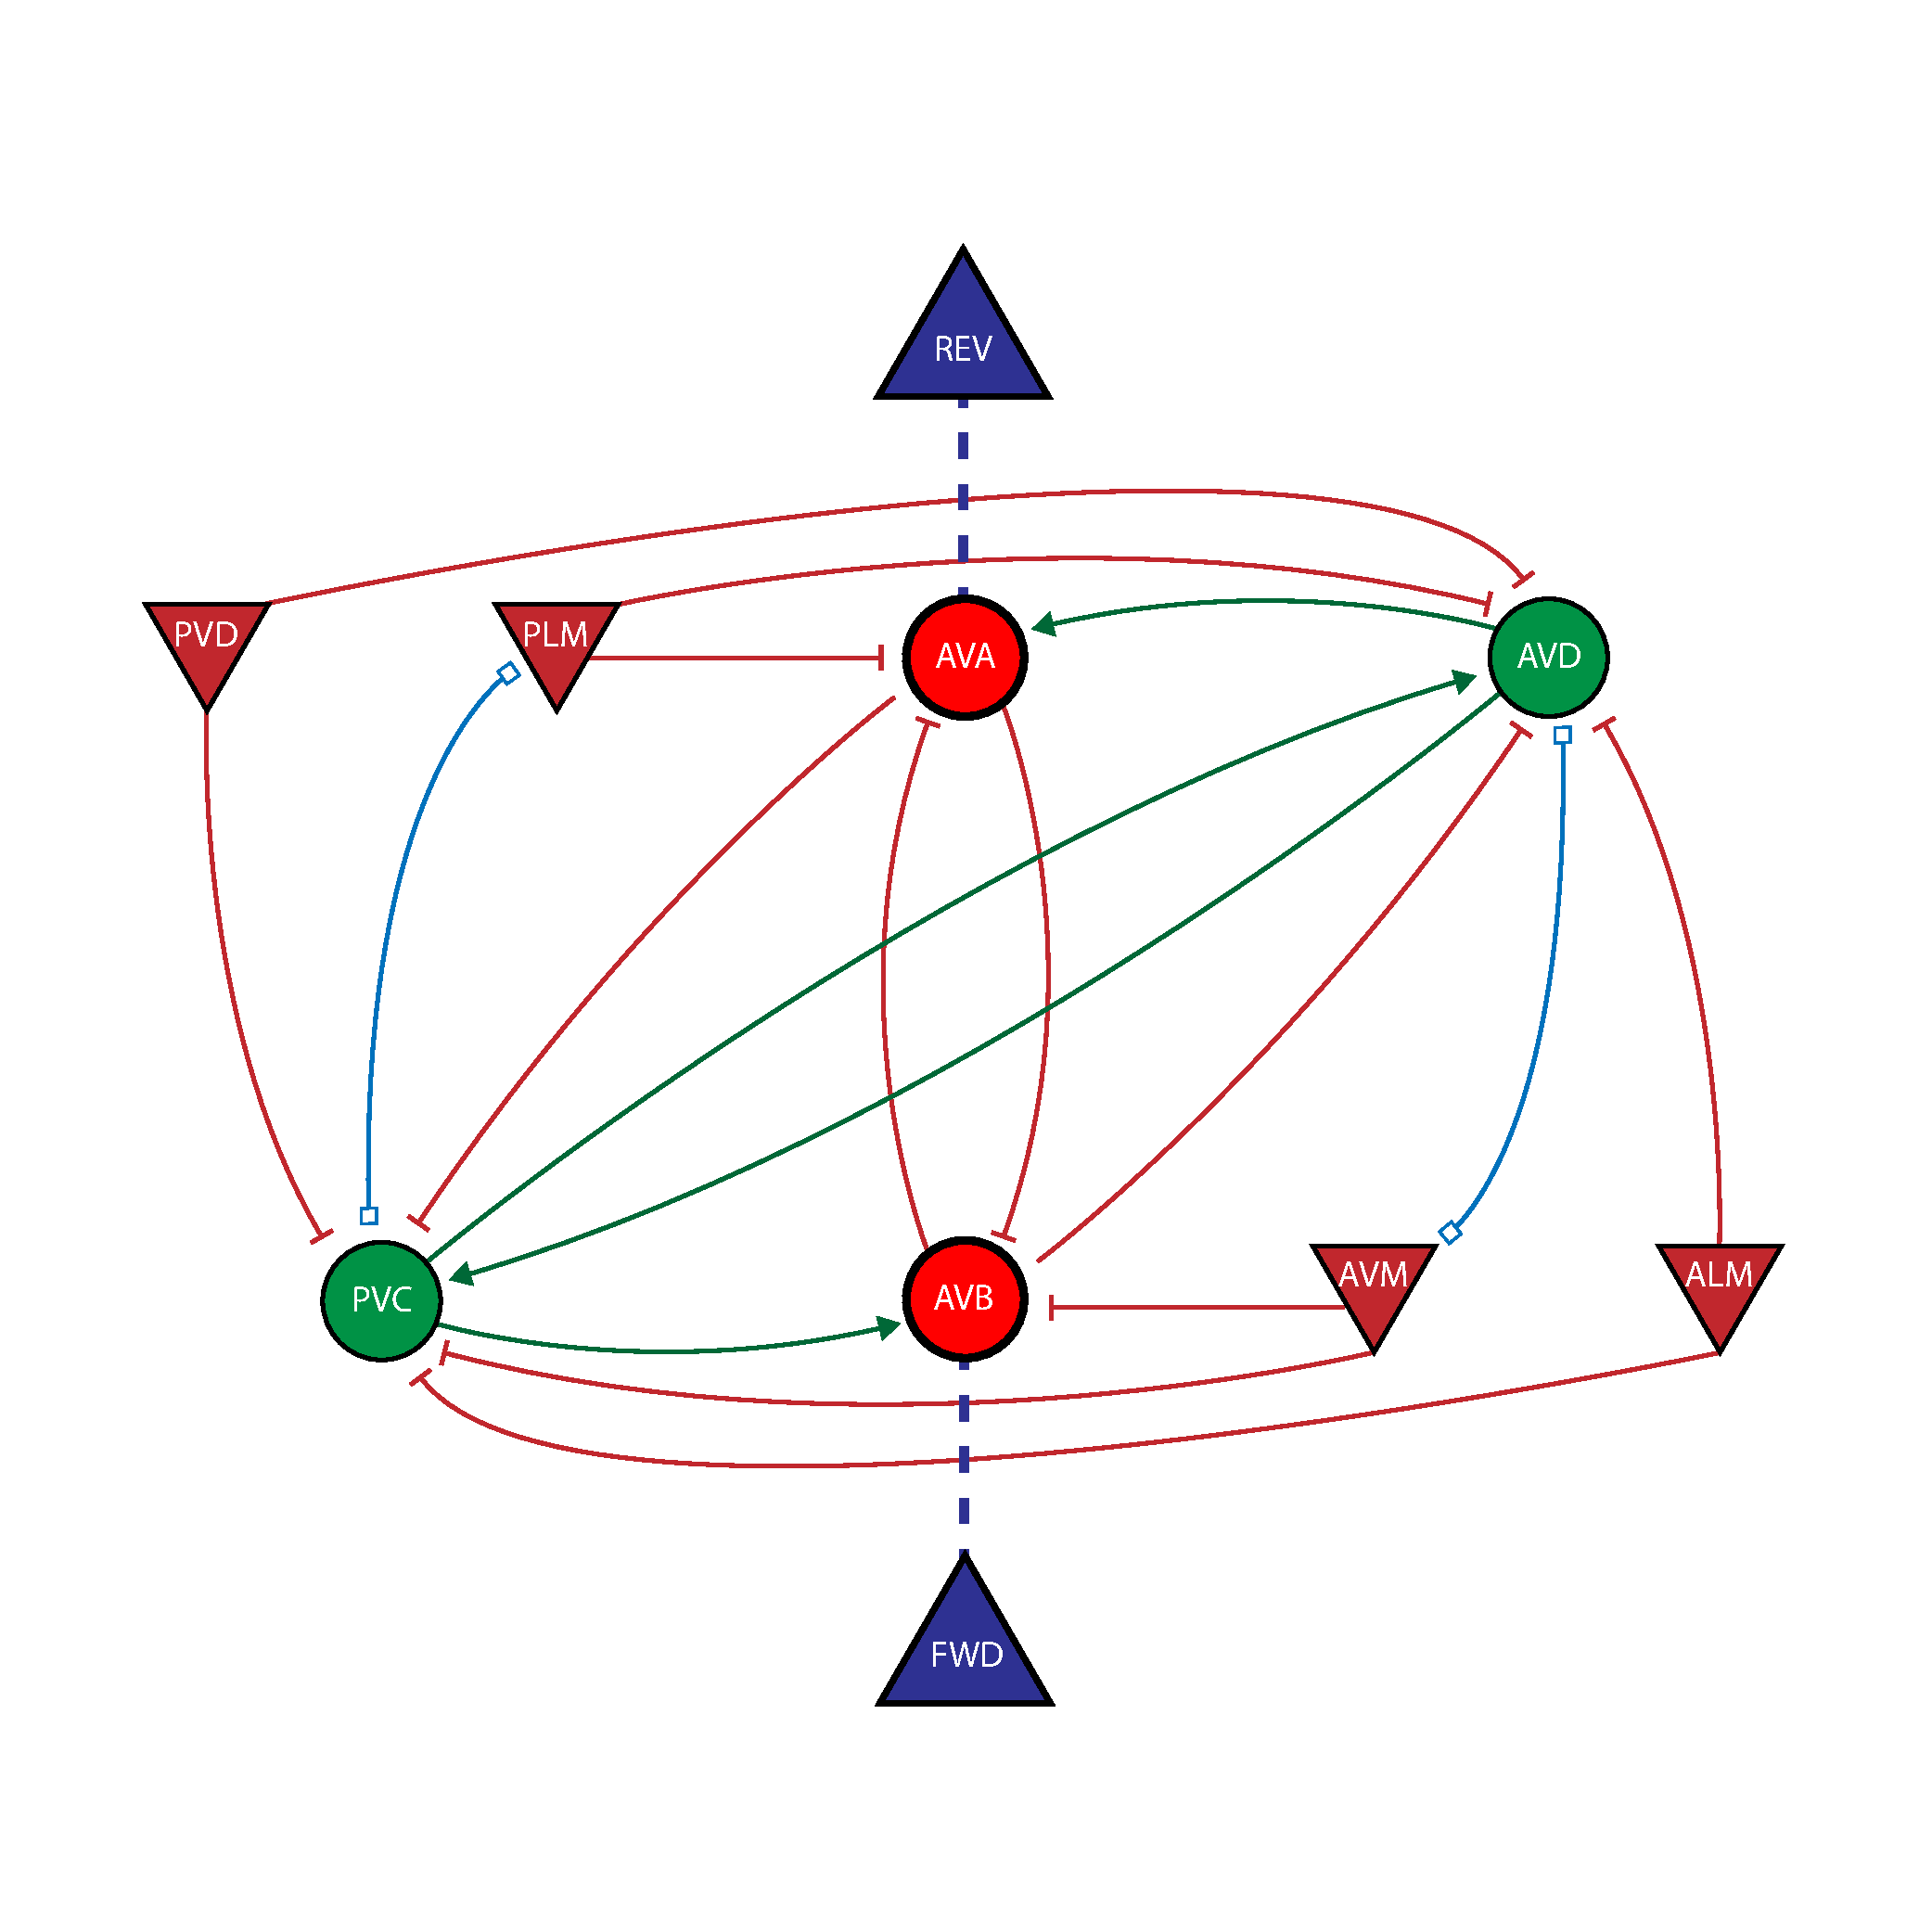
\includegraphics[width=6.5cm]{figures/Neural_Net_v3_ohneLegende.pdf}
			\caption{Biologisches neuronales Netz des \textit{C. Elegans}.}
			\label{fig:bnn_celegans}
		\end{figure}
	\end{column}
	\hspace{-1cm}
	\begin{column}{0.5\textwidth}
		\vspace{1.1cm}
		\begin{figure}[H] %[!t] ...
			\centering
			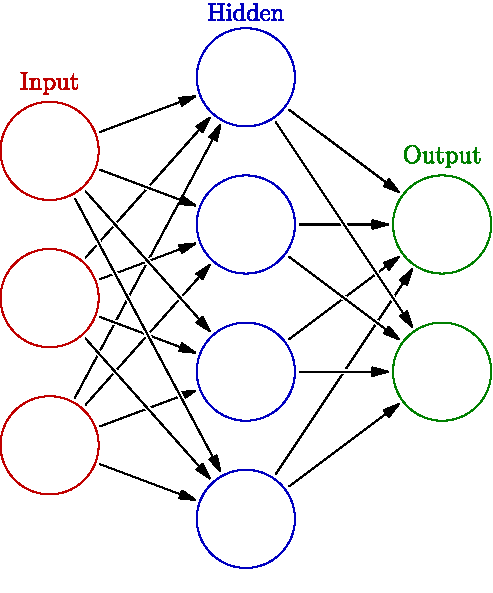
\includegraphics[width=4.5cm]{figures/Colored_neural_network.pdf}
			\caption{Modell eines künstlichen neuronalen Netzes}
			\label{fig:model_knn}
		\end{figure}
	\end{column}
\end{columns}
\end{frame}

% =======================

\begin{frame}

	\frametitle{\ChapterBackup}
	\framesubtitle{Herleitung des Leaky Integrate and Fire - Modells (1/3)}
	\vspace{0.3cm}
	Um eine geeignete Differenzialgleichung herzuleiten, wird zuerst das erste Kirchhoffsche Gesetz angewendet
	\begin{align}
	\label{eq:lif_current}
	I = I_R + I_C\text{.}
	\end{align}
	Der Strom $I_R$ ist einfach durch das Ohmsche Gesetz wie folgt zu berechnen
	\begin{align}
	\label{eq:lif_IR}
	I_R = \frac{U_R}{R} = \frac{U - U_{Leak}}{R}\text{.}
	\end{align}
	Der Strom $I_C$ wird durch die Definition eines Kondensators $C_m = \tfrac{q}{U}$ zum kapazitiven Strom 
	\begin{align}
	\label{eq:lif_IC}
	I_C = \frac{dq}{dt} = C_m \frac{dU}{dt}\text{.}
	\end{align}
	Hierbei steht $q$ für die elektrische Ladung und $U$ für die anliegende Spannung.\\
	Einsetzen von \eqref{eq:lif_IR} und \eqref{eq:lif_IC} in \eqref{eq:lif_current} ergibt
	\begin{align}
	\label{eq:lif_I}
	I = \frac{U - U_{Leak}}{R} + C_m\frac{dU}{dt}\text{.}
	\end{align}
\end{frame}

% =======================

\begin{frame}
	\frametitle{\ChapterBackup}
	\framesubtitle{Herleitung des Leaky Integrate and Fire - Modells (2/3)}
	\vspace{0.3cm}
	Wird diese Gleichung mit $R$ multipliziert und umgestellt, bildet sich die folgende lineare Differenzialgleichung erster Ordnung:
	\begin{align}
	\label{eq:lif_nd}
	R C_m \frac{dU}{dt} = (U_{Leak} - U) + R I\text{.}
	\end{align}
	Der Strom $I$ wird als Eingangsgröße verstanden und im weiteren Verlauf als $I_{in}$ betitelt. Nach Division durch $RC$ und Einführung des Leitwerts $G_{Leak} = \tfrac{1}{R}$ entsteht die gewollte Form:
	\begin{align}
	\label{eq:lif}
	\frac{dU}{dt} = \frac{G_{Leak}(U_{Leak} - U) + I_{in}}{C_m}\text{.}
	\end{align}
	In dieser Gleichung stehen die Variablen $G_{Leak}$, $U_{Leak}$ und $C_m$ für Parameter der betrachteten Nervenzelle, während $I_{in}$ stellvertretend für alle eingehenden Ströme aus Stimuli, chemischen Synapsen und Gap-Junctions steht
	\begin{align}
	\label{eq:lif_current_in}
	I_{in} = \sum_{i = 1}^{n}{I_{Stimuli}} + \sum_{i = 1}^{n}{I_{Syn}} + \sum_{i = 1}^{n}{I_{Gap}}\text{.}
	\end{align}
\end{frame}

% =======================

\begin{frame}
	\frametitle{\ChapterBackup}
	\framesubtitle{Herleitung des Leaky Integrate and Fire - Modells (3/3)}
	\vspace{0.3cm}
	Die anliegenden Synapsenströme sind durch folgenden formularen Zusammenhang zu berechnen:
	\begin{align}
	\label{eq:chem_syn_current}
	I_{Syn} = \frac{w}{1 + \exp^{\sigma(u_{pre} + \mu)}}(E - u_{post})\text{.}
	\end{align}
	Synapsenströme sind grundsätzlich von den pre- und postsynaptischen Potentialen der jeweiligen Nervenzellen $u_{pre}$ und $u_{post}$ abhängig. Weiterhin können diese chemischen Synapsen exzitatorisch oder inhibitorisch wirken. Diese Eigenschaft wird durch das sog. Nernstpotential $E\in[-90\text{ mV}, 0\text{ mV}]$ beschrieben. Weitere Größen dieser Gleichung bilden die Kreisfrequenz $w$, die Standardabweichung $\sigma$ und der Erwartungswert $\mu$.\\
	Gap-Junctions bilden die Ausnahme, denn sie dienen als Ausgleichsglied und wirken bidirektional. Ihr Strom wird wie folgt berechnet:
	\begin{align}
	\label{eq:gap_syn_current}
	I_{Gap} = \hat{w}(u_{post} - u_{pre})\text{.}
	\end{align}
	Für die Berechnung des Gap-Junction Stroms benötigt es ebenfalls das pre- und postsynaptische Potenzial der jeweiligen Nervenzellen $u_{pre}$ und $u_{post}$, sowie die Kreisfrequenz $\hat{w}$.
\end{frame}

% =======================

\begin{frame}
	\frametitle{\ChapterBackup}
	\framesubtitle{Aktionsraum und Übersetzungsvorschrift der Sensor-Neuronen}
	\vspace{0.3cm}
	Um die jeweiligen Größen durch die Sensorneuronen zu übersetzen, werden folgende Funktionen für die jeweils positive und negative Sensorneurone $S_{positiv}$ und $S_{negativ}$ angenommen:
	\begin{align}
	\label{eq:sensor_translation_p}
	S_{positiv} &:= \begin{cases}-70\text{ mV} & x\leq 0\\-70\text{ mV} + \frac{50\text{ mV}}{x_{min}}x & 0 < x \leq x_{min} \\-20\text{ mV} & x > x_{max}  \end{cases}\\
	\label{eq:sensor_translation_n}
	S_{negativ} &:= \begin{cases}-70\text{ mV} & x\geq 0\\-70\text{ mV} + \frac{50\text{ mV}}{x_{min}}x & 0 > x \geq x_{min} \\-20\text{ mV} & x < x_{max}  \end{cases}
	\end{align}
	$x\in[x_{min}, x_{max}]$ ist eine messbare, dynamische Systemvariable, welche in den gegebenen Grenzen $x_{min} $ und $x_{max}$ auftritt. Lediglich eine Fallunterscheidung wird getroffen: nimmt $x$ einen positiven Wert an, wird Sensorneurone $S_{positiv}$ aktiviert, bei negativem $x$-Wert, agiert die Sensorneurone $S_{negativ}$.
\end{frame}

% =======================

\end{document}

%%% Local Variables:
%%% mode: latex
%%% TeX-master: t
%%% End:
